%======================================================
% Technische Universitaet Darmstadt
% Fachbereich Elektrotechnik und Informationstechnik
% Fachbereich Informatik (Zweitmitglied)
% Fachgebiet Multimedia Kommunikation (KOM)
% Prof. Dr.-Ing. Ralf Steinmetz
%======================================================
% Template for KOM Theses
% VERSION 1.5 (July 2020)
% Use pdfLaTeX (others not supported)
% Contact at KOM: Julian Zobel (julian.zobel@...)
%======================================================
% READ THE README FIRST!
%======================================================
%
% add pdfa to [ ] for pdfa document!
%
\documentclass[11pt,longdoc,accentcolor=tud1b,paper=a4]{tuddesign/tudreport}
%======================================================
% KOM-Blau = accentcolor=tud1b		
% Grau = accentcolor=tud0a 
%======================================================

%======================================================
% General package loading and definitions
%======================================================
\usepackage[utf8]{inputenc}
\usepackage{textcomp} 
% \usepackage{ngerman}
\usepackage[american,ngerman]{babel}
\usepackage{xspace}
\usepackage[fleqn]{amsmath} % math environments and more by the AMS 

\newcounter{dummy} % necessary for correct hyperlinks (to index, bib, etc.)
\newcommand{\myfloatalign}{\centering} % how all the floats will be aligned

%======================================================
% KOM-modifications of the TUD-layout
%======================================================
% reduce font size of page footers and headers (fancyhdr)
\renewcommand{\footerfont}{\fontfamily{\sfdefault}\fontseries{m}\fontshape{n}\footnotesize\selectfont}
% remove space between items 
\usepackage{enumitem}
	\setenumerate{noitemsep}
	\setitemize{noitemsep}
	\setdescription{noitemsep}
%\setlist{nolistsep}

%======================================================
% Package loading for example contents (content.tex)
%======================================================
\usepackage{algorithm}
\usepackage{algpseudocode}
\usepackage{wrapfig}
\usepackage{tabularx} % better tables
\setlength{\extrarowheight}{3pt} % increase table row height
\usepackage{booktabs}
\usepackage{caption}
\captionsetup{format=hang,font=small}
\usepackage[square,numbers]{natbib}
%\usepackage{subfig}
\usepackage{subcaption}
\usepackage[stable,bottom]{footmisc}
\usepackage{framed}
\usepackage{color}

%======================================================
% Flags
%======================================================
\newboolean{final} %Deklaration
\setboolean{final}{false} %Zuweisung

\newboolean{showTranslationOnTitle} %Deklaration
\setboolean{showTranslationOnTitle}{false} %Zuweisung

\newboolean{showEnglishThesisStatement} %Deklaration
\setboolean{showEnglishThesisStatement}{false} %Zuweisung

%======================================================
% Important information: to be set here and only here
%======================================================

% Title of the thesis in DE or EN, depending on thesis language
\newcommand{\komTitle}{Entwicklung von Methoden und Konzepten für ein spielerisches Trainingsprogramm zur Gehörbildung\xspace} 
% Translation of the title in either DE or EN, depending on thesis language
\newcommand{\komTitleTranslation}{Development of methods and concepts for a game-based ear training program\xspace}

% Typ der Arbeit: Diplomarbeit Studienarbeit Master-Thesis Bachelor-Thesis
\newcommand{\komThesisType}{Bachelor-Thesis\xspace} 

% Studiengang: Elektrotechnik und Informationstechnik, Informationssystemtechnik, Informatik, ...
\newcommand{\komCourseOfStudy}{Informatik\xspace}

\newcommand{\komName}{Lukas Rohde\xspace}
\newcommand{\komSubmissionDate}{15. Juli 2021\xspace}% use only this date format

\newcommand{\komGutachter}{Gutachter: Prof. Dr.-Ing. Ralf Steinmetz\xspace}
\newcommand{\komBetreuer}{Betreuer: Dr.-Ing. Stefan Göbel\xspace}
\newcommand{\komExternerBetreuer}{}
\newcommand{\komID}{KOM-type-number\xspace}



%======================================================
% Setup for hyperref
%======================================================
\usepackage[pdftex,hyperfootnotes=true,pdfpagelabels]{hyperref}
	\pdfcompresslevel=9
	\pdfadjustspacing=1 
\hypersetup{%
    colorlinks=false, linktocpage=false, pdfstartpage=1, pdfstartview=FitV,%
    breaklinks=true, pdfpagemode=UseNone, pageanchor=true, pdfpagemode=UseOutlines,%
    plainpages=false, bookmarksnumbered, bookmarksopen=true, bookmarksopenlevel=1,%
    hypertexnames=true, pdfhighlight=/O, %nesting=true,%frenchlinks,%
    %urlcolor=tud1b, linkcolor=tud1b, citecolor=tudtud1bccent,
    pdftitle={\komTitle, \komThesisType, \komID},%
    pdfauthor={\komName, KOM, TU Darmstadt},%
    pdfsubject={},%
    pdfkeywords={},%
    pdfcreator={},%
    pdfproducer={}%
}

%============================================
% Setup of the title page (do not change)
%============================================

\title{\komTitle}
\ifthenelse{\boolean{showTranslationOnTitle}}{\subtitle{\komTitleTranslation \\ \komThesisType}}{\subtitle{\komThesisType}}		
\subsubtitle{\komName \\ \komID}
\institution{\raggedleft Fachbereich Elektrotechnik \\und Informationstechnik\\%
	Fachbereich Informatik (Zweitmitglied)\\[\baselineskip]%
	Fachgebiet Multimedia Kommunikation \\%(KOM)
	Prof. Dr.-Ing. Ralf Steinmetz}


%============================================
% Setup of the title backside (do not change)
%============================================
\lowertitleback{%
	Technische Universität Darmstadt \\%
	Fachbereich Elektrotechnik und Informationstechnik\\%
	Fachbereich Informatik (Zweitmitglied)\\[\baselineskip]%
	Fachgebiet Multimedia Kommunikation (KOM)\\%
	Prof. Dr.-Ing. Ralf Steinmetz%
	%Department of Electrical Engineering and Information Technology \\%
	%Department of Computer Science (Adjunct Professor) \\[\baselineskip]%
	%Multimedia Communications Lab (KOM) \\%
	%Prof. Dr.-Ing. Ralf Steinmetz %
}


\uppertitleback{%
    \textbf{\komTitle} \\%
    \komTitleTranslation \\[\baselineskip]%
	\komThesisType \\%
    Studiengang: \komCourseOfStudy \\%
	\komID \\[\baselineskip]%
	Eingereicht von \komName \\%
	Tag der Einreichung: \komSubmissionDate \\[\baselineskip]%
	\komGutachter \\%
	\komBetreuer \\%
	\komExternerBetreuer%
}
	
%======================================================
% MAIN DOCUMENT STARTS HERE
%======================================================
\begin{document}
	
	\colorlet{tudidentbar}{tud1b} %first page colored - DO NOT MODIFY THIS
	%======================================================
	% The front matter
	%======================================================
	\pagenumbering{roman}
	\frenchspacing
	\raggedbottom
	\selectlanguage{ngerman} % american ngerman
	\maketitle
	
	%
	
	% identbar color for the rest of the thesis - DO NOT MODIFY THIS
	\colorlet{tudidentbar}{tud0b} 
    
    \begin{otherlanguage}{ngerman}
    
    \chapter*{Erklärung zur Abschlussarbeit gemäß § 22 Abs.\ 7 und § 23 Abs.\ 7 APB der TU Darmstadt}	 
    
    Hiermit versichere ich, \komName, die vorliegende \komThesisType gemäß § 22 Abs. 7 APB der TU Darmstadt ohne Hilfe Dritter und nur mit den angegebenen Quellen und Hilfsmitteln angefertigt zu haben.
    Alle Stellen, die Quellen entnommen wurden, sind als solche kenntlich gemacht worden. 
    Diese Arbeit hat in gleicher oder ähnlicher Form noch keiner Prüfungsbehörde vorgelegen. \\
   
	\noindent Mir ist bekannt, dass im Falle eines Plagiats (§38 Abs.2 APB) ein Täuschungsversuch vorliegt, der dazu führt, dass die Arbeit mit 5,0 bewertet und damit ein Prüfungsversuch verbraucht wird. 
	Abschlussarbeiten dürfen nur einmal wiederholt werden.\\

	\noindent Bei der abgegebenen Thesis stimmen die schriftliche und die zur Archivierung eingereichte elektronische Fassung gemäß §~23 Abs.~7 APB überein. \\

	%%%
	% IF ENGLISH TEXT WISHED OR REQUIRED, SET THE FLAT TO TRUE (see above)
	%%%
	\ifthenelse{\boolean{showEnglishThesisStatement}}{
	
	\vspace{2em}
	\noindent English translation for information purposes only: \\
	
	\noindent \textbf{Thesis Statement pursuant to § 22 paragraph 7 and § 23 paragraph 7 of APB TU Darmstadt} \\
	
	\noindent I herewith formally declare that I, \komName, have written the submitted thesis independently pursuant to § 22 paragraph 7 of APB TU Darmstadt. 
	I did not use any outside support except for the quoted literature and other sources mentioned in the paper. 
	I clearly marked and separately listed all of the literature and all of the other sources which I employed when producing this academic work, either literally or in content.
	This thesis has not been handed in or published before in the same or similar form. \\

	\noindent I am aware, that in case of an attempt at deception based on plagiarism (§38 Abs. 2 APB), the thesis would be graded with 5,0 and counted as one failed examination attempt. 
	The thesis may only be repeated once. \\
	
    \noindent In the submitted thesis the written copies and the electronic version for archiving are pursuant to § 23 paragraph 7 of APB identical in content.
    
	}{}	
    \vspace{4em}
    
    \noindent Darmstadt, den \komSubmissionDate 
    
    \vspace{3em}
    
    \noindent\rule{5cm}{0.4pt}
    
    \noindent\komName
    
    \end{otherlanguage}
   
	\tableofcontents
	\listoffigures
	%\listoftables
	
	%======================================================
	% The main matter (insert your contents here)
	%======================================================
	\cleardoublepage
	\pagenumbering{arabic}

	
\newcommand{\hint}[1]{
  \ifthenelse{\boolean{final}}{}{
\textcolor{green}{   
	\begin{framed}
	\noindent
	\underline{Hint:}\\ \newline
	#1
	\end{framed}
}
}}
	%! Suppress = MissingLabel
\begin{abstract}
    In der folgenden Arbeit werden zunächst die wichtigsten Anwendung zur Gehörbildung analysiert und auf ihre wichtigsten Punkte hin untersucht. Daraufhin werden einige Ansätze zur algorithmischen Erkennung von Tönen untersucht und auf ihre Tauglichkeit im Kontext einer echtzeit Anwendung untersucht. Basierend auf diesen Ergebnissen wird anschließend eine Trainingsanwendung zur Schulung des Gehörs konzeptioniert, sowie ein Algorithmus zur Tonerkennung im Umfeld von Unity. Die Ergebnisse werden anschließend mit drei Gruppen evaluiert und ausgewertet hinsichtlich der Tauglichkeit der Anwendung als Trainingsprogramm und Unity als Basis für dieses. Zuletzt wird ein Fazit gezogen und auf mögliche zukünftige Anwendungsgebiete eingegangen.
\end{abstract}

%TODO Roter Faden immer am ende des Kapitels das nächste aufgreifen
% in konzeption ruhig genauere kapitel aufgliederung
% maximal 1 seite ohne überschrift irgendeiner art


\chapter{Einleitung}
Im Allgemeinen unterscheidet man zwischen dem sogenannten absoluten Gehör und dem relativen Gehör. Während eine Person mit einem absoluten Gehör eine Note ohne eine Referenz und nur mit ihrem Gehör bestimmen kann, kann eine Person, welche nur ein ausgebildetes relatives Gehör hat, eine Note nur mit einem Vergleichston bestimmen. Wichtig ist, dass die meisten Menschen das relative Gehör trainieren können, wohingegen man das absolute Gehör nicht trainieren kann \cite{gussmack2006latentes}. Will man das relative Gehör trainieren, so hat man die Wahl zwischen verschiedenen Übungsansätzen und Methoden. Unter diese Methoden fallen beispielsweise das Erhören und Vervollständigen von Intervallen oder Akkorden. Weiterhin werden häufig Diktate verwendet um das relative Gehör weiter zu schulen, wie etwa in einem Melodiediktat, wo die lernende Person die richtigen Noten einer gehörten Melodie aufschreiben muss. Ein großer Aspekt ist auch, dass die Lernenden nicht nur Töne, Intervalle, Akkorde und Melodien erkennen, sondern auch reproduzieren können. Das Reproduzieren kann dabei heißen, dass ein Intervall gesungen werden muss oder ein Akkord vervollständigt werden soll. Die Fähigkeit, all das reproduzieren zu können ist vor allem im Zusammenspiel verschiedener Musiker und Musikerinnen wichtig. Dirigenten und Orchesterleiter sind ebenfalls auf ihre Fähigkeiten angewiesen, Intervalle Akkorde oder Melodien vorsingen zu können um so den Musikern die gewollten musikalischen Ideen vermitteln zu können. 

\section{Motivation}
\emph{
    \glqq 
    Study of music and
    its literature presupposes the ability to hear,
    read, and write the language. Lacking this ability one is
    comparatively helpless and dependent. This perfectly
    obvious truth is universally accepted without question
    in the study of every language excepting music. Teachers, capable otherwise, allow and encourage the serious
    study of music by students who do not comprehend what
    they hear. Ability to hear is the essence of music, the
    core of education in music is ear training
  ''  \cite{spencer1947ear}
} \\
Herbert S. Spencer beschreibt in einem Artikel von 1947 die Notwendigkeit der Gehörbildung um Musik in vollen Zügen wahrnehmen und ausüben zu können. Er setzt dabei das Hören von Musik mit dem Lernen von Sprachen gleich, wobei er feststellt, dass einzig in der Lehre der Musik kaum Wert auf das Hören dieser gelegt wird. Er sieht darin einen großen Verlust und beschreibt einen Musiker ohne ausgebildetes Gehör als vergleichsweise hilflos und abhängig. \\
Obwohl Gehörbildung bereits seit langer Zeit von Musikern als wichtig für das Musizieren wahrgenommenen wird, findet die Förderung dieser heutzutage häufig nur im Studium der Musik statt. Weiterhin sitzt zum Schulen des Gehörs häufig noch ein Lehrer an einem Klavier, welcher etwas vorspielt und die Schüler ihm zuhören und das Gehörte aufschreiben müssen. Der Unterricht der Gehörbildung ist dementsprechend nicht allgemein zugänglich für die breite Masse der Musiker und stark beschränkt auf die Umgebung des studentischen Seminarsaals. Es existieren bereits einige Programme, welche bei dem Schulen des Gehörs der lernenden Person helfen, jedoch nicht das Singen ermöglichen. 
Ziel dieser Arbeit soll sein, die existierenden Trainingsprogramme zur Gehörbildung auf ihre wichtigsten Aspekte hin zu untersuchen und basierend auf den Ergebnissen der Analyse ein prototypisches Trainingsprogramm mithilfe von Unity3D zu entwickeln, welches die wesentlichen Aspekte der vorhandenen Software aufgreifen und verbessern soll. Das entwickelte Programm soll bestenfalls sowohl auszubildende Musiker im Studium unterstützen, als auch Amateurmusiker in der Fortbildung des Gehörs fördern. Unity bietet keine integrierte Funktion um echtzeit Tonverarbeitung zu implementieren, weshalb die Tonerkennung eine besondere Herausforderung sein wird. Weiterhin muss ein ansprechendes User Interface sowohl für Amateurmusiker, als auch (auszubildende) professionelle Musiker entwickelt werden. 

\section{Aufbau der Arbeit}
Im nächsten Kapitel werden zunächst einige wichtige Definitionen zu den Oberthemen der Signalverarbeitung, Musiktheorie und zu Serious Games gegeben, welche für das restliche Verständnis der Arbeit wichtig sind. Daraufhin werden im dritten Kapitel die aktuell eingesetzten Programme zur Gehörbildung vorgestellt und hinsichtlich vorher definierten Gesichtspunkten analysiert. Im zweiten Teil des dritten Kapitels werden außerdem bekannte Methoden zur Tonerkennung und zur echtzeit Eingabe von Ton in Unity analysiert. Basierend auf den Erkenntnissen des dritten Kapitels, wird im darauffolgenden vierten Kapitel ein Trainingsprogramm zur Gehörbildung mit Unity konzipiert. Die Konzeption ist dabei aufgeteilt in den Entwurf des Spiels aus der Sicht des Nutzers (user-centered design), den Entwurf der Systemkomponenten und der Tonerkennung sowie dem Evaluationskonzept. Im fünften Kapitel wird die Implementierung des Trainingsprogramms in Unity vorgestellt und im Detail auf die implementierten Funktionen eingegangen. Das sechste Kapitel beleuchtet die Evaluationsschritte näher, wobei auch auf die Vorbereitung und die Durchführung der Evaluation eingegangen wird. Außerdem werden die Ergebnisse der Evaluation analysiert und ausgewertet. Im letzten Kapitel wird schließlich ein Fazit gezogen, sowie ein Ausblick auf mögliche erweiternde Funktionen, sowie weitere Anwendungsbereiche gegeben.
%- Thema
%- Warum relevant? Wie ist es einzuordnen? (Singen macht Spaß -> Problem: Viele haben keine ausgeprägte gehörbildung, Training für Lernende)
%- Motivation: Viele haben Schwierigkeit Gehörbildung anständig zu lernen (fehlende Programme, schlechte Handhabung, festes Lernkit)
%- Allg. Fragestellung: "Viele Menschen haben Probleme..., Wollen Lernen..., Müssen im Rahmen ihres Studiums lernen..."
%- techn. Problemstellung: "Realtime Soundverarbeitung unter UNity mit angemessener Fehlerquote / Intuitives Design der Notenausgabe/Platzierung auf das Notensystem"
%Introkapitel
%- Thema beschreiben 
%- Problemstellung grob eingehen
%-- facettenreiche und betrifft die folgenden gebiete
%--- serious games, audio, Grundlagen..
%y-- als nächstes schau ich das näher an -> rundown der arbeit geben



\chapter{Grundlagen}
\section{Signalverarbeitung}
%- Frequenz
%- Abtasttheorem
%- FFT
%- Unity eingebauten Methoden
\subsection*{Nyquist-Shannon-Abtasttheorem}
\label{sec:Abtast}
Das Nyquist-Shannon-Abtasttheorem besagt, dass eine Frequenz $f_{max}$ nur dann exakt rekonstruiert werden kann, wenn es mit einer mindestens doppelt so hohen Frequenz $2f_{max}$ abgetastet wird. Auf die Akustik bezogen heißt das, dass man um eine Frequenz von beispielsweise 20kHz ohne Verlust aufzunehmen, man den Ton mit mindestens 40kHz \glqq abtasten'' muss. Abtasten heißt hier, den aktuellen Wert bzw. Frequenz zu speichern. 

\subsection*{Fouriertransformation}
\label{sec:Fouriertransformation}
Eine Fouriertransformation ist eine Methode, mit der man ein zeitabhängiges Signal in den Frequenzraum überführen kann. Das Ergebnis ist ein frequenzabhängiges Spektrum.
Da sich bei einem Ton ein bestimmtes Muster über einen endlichen Zeitraum wiederholt, handelt es sich um ein periodisches Signal. Es muss demnach möglich sein, dieses periodische Signal mithilfe von Sinuswellen zu modellieren. Untersucht man die entstandene Funktion, so kann man die im Signal vorhandenen Frequenzen herausfiltern bzw. erkennen. Diese Eigenschaft ist offensichtlich essenziell bei der Tonerkennung. Eine Fouriertransformation setzt eine ganzzahlige Periode voraus, sodass diese nicht von der Analyse abgeschnitten wird. Das Abschneiden einer Periode hat zur Folge, dass das entstehende Spektrum ungenau wird.
Dieses Problem kann durch Fensterfunktionen gelöst werden. Durch Fensterfunktionen werden die Amplituden an den Flanken weich gezeichnet, sodass die Endpunkte der Perioden aneinander angeglichen werden und es zu keinen unstetigen Übergängen kommt \cite{Butz2006}.

\section{Musiktheorie}
\subsection*{Intervalle}
\label{sec:Intervalle}
Ein Intervall im musikalischen Sinne bezeichnet den Abstand zwischen zwei Tönen. Man kann in der Spielpraxis zwischen den sogenannten harmonischen Intervallen und den melodischen Intervallen unterscheiden. Bei den harmonischen Intervallen erklingen die Töne gleichzeitig, wohingegen bei melodischen Intervallen die Töne hintereinander erklingen. Intervalle lassen sich mathematisch als Proportionen der erklingenden Töne zueinander beschreiben, das wichtigste Intervall ist hierbei die Oktave. Die Oktave hat ein Frequenzverhältnis von 2:1, 
sie entspricht also immer der doppelten Frequenz von einem Ton zu dem Anderen. Wie die Tonabstände innerhalb einer Oktave aufgeteilt werden, ist zwischen den Tonsystem unterschiedlich. Alle dieser Unterteilungen benennen die Schritte innerhalb einer Oktave nach den lateinischen Ordinalzahlen, wobei Oktave Acht bedeutet. Wie der Name Oktave also schon vermuten lässt, liegen innerhalb einer Oktave sieben andere Intervalle. Neben den Namensbestimmungen durch die Ordinalzahlen, gibt es ebenfalls die Zusätze von vermindert und übermäßig. Diese weitere Einstufung der Intervalle ermöglicht es Intervalle mit einem halben Ton abstand zu notieren, neben den Ganztönen. Berücksichtigt man all das, so lässt sich eine Oktave in 
12 Halbtöne aufteilen, wobei jeder mögliche Abstand zwischen diesen Halbtönen benannt werden kann. \\\\
Es gibt neben den Einteilungen von Intervallen innerhalb einer Oktave auch Bezeichnungen für Intervalle, welche einen Abstand größer als eine Oktave umspannen. Ich möchte diese aufgrund der Vollständigkeit auch erwähnen, jedoch werden diese nicht weiter in der folgenden Arbeit berücksichtigt.
Diese Intervalle folgen weiterhin der lateinischen Ordinalzahlreihe, sodass ein Intervall, welches einen Ganzton weiter umspannt als die Oktave, dementsprechend None genannt wird. \cite{abcmusik}

\subsection*{Die Grundfrequenz und Obertöne}
\label{sec:Oberton} \label{sec:Nebenschwingung} \label{sec:Grundfrequenz}
Bei allen musikalisch erzeugten Tönen treten neben dem sogenannten Grundton bzw. der Grundfrequenz auch Nebenschwingungen oder Obertöne mit auf.
Bei der Grundfrequenz handelt es sich um die tiefste auftretende Schwingung in diesem Spektrum, die restlichen messbaren Schwingungen sind die sogenannten Obertöne, diese bestimmen vor allem die Klangfarbe, verändern aber nicht den erklingenden Ton in seiner Höhe.
In der Musik bestimmt also die Grundfrequenz den wahrgenommenen erklingenden Ton und die Obertöne nur die Wahrnehmung des Tons. Die Obertöne können dabei aber häufig einen stärkeren Ausschlag verursachen, untersucht man einen Ton mithilfe
einer Fouriertransformation. Ein Ton im musikalischen Sinn beschreibt also nicht eine reine Sinuswelle, sondern vielmehr eine überlagerung mehrerer Schwingungen, welche zusammen den Ton mit Klangfarbe ausmachen. Obertöne sind in der Regel ganzzahlige vielfache 
des Grundtons, Töne mit dieser Eigenschaft nennt man Harmonisch. Ausnahmen zu dieser Regel sind vor allem Klänge welche für das menschliche Ohr als unschön oder störend empfunden werden, wie
beispielsweise Glocken oder fallende Rohre und Stangen, sie werden auch unharmonisch genannt. \cite{abcmusik} \cite{harmonische_obertne}


\subsection*{Tonsysteme und Stimmung}
\label{sec:Tonsysteme}
Wie bereits in \ref{sec:Intervalle} angesprochen, gibt es verschiedene Systeme um die Tonabstände zu bestimmen, ich möchte hier nun die wichtigsten Systeme beleuchten und auf ihre Anwendungen und Herkünfte eingehen.
Verschiedene Arten von Unterteilungen werden auch Stimmungen genannt. Betrachten wir zunächst den Tonraum, in welchem wir uns befinden. \\
In dem geordneten Tonraum lässt sich jedem Ton genau eine Frequenz zuordnen, wobei gilt, um so höher die Frequenz, desto höher ist auch der erklingende Ton. Außerdem ist jedem Paar von Tönen $t_1, t_2$ bzw. Frequenzen $f_1, f_2$ genau ein Intervall $i_{12}$ zugeordnet, 
wir können daraus folgern, dass das Intervall der Töne, ein Frequenzverhältnis von $f_2 : f_1$ hat. Es wird außerdem in der Musik die Einheit Cent herangezogen um genauere Angaben zu verschieden hohen Tönen zu machen. Ein Cent ist definiert als 
$1/1200$ Oktave. Betrachtet man den Raum der Intervalle und der Frequenzverhältnisse, so fällt auf, dass ein Homomorphismus zwischen diesen beiden Räumen gegeben ist. Addiert man zwei Intervalle im Intervallraum, so multipliziert man deren Frequenzverhältnisse bzw. Proportionen. \\
Ein kurzes Beispiel soll diesen Zusammenhang verdeutlichen. Nehmen wir die kleine Terz $i_1 =  316$ Cent und die Quinte $i_2 =  701$ Cent und ihre dazugehörigen Frequenzverhältnisse $p_1 = 6/5$ und $p_2 = 3/2$ als gegeben an.
$$    i = i_1 + i_2 = 1017  $$
$$    p = p_1 * p_2 = 9/5   $$
$$   => 1200 * \log_2{9/5} \approx 1017     $$
\\
Es gibt nun verschiedene Verhältnisse, welche verschiedene sogenannte Stimmungen bilden. Zu den bekanntesten Stimmungen zählen die reine Stimmung, die pythagoreische Stimmung und die gleichstufige Stimmung.
All diese Stimmungen haben die Gemeinsamkeit, dass sie durch Cent beschrieben werden und somit alle eine Oktave als 1200 Cent bzw. als ein Stimmungsverhältnis von 1:2 definieren. Die Unterschiede der Stimmungen ergeben sich dann, in welchen Frequenzen die einzelnen Töne zwischen den Oktaven definiert sind. Die älteste Stimmung aus dem europäischen Raum ist die pythagoreische Stimmung. Pythagoras reihte für die Berechnung zwölf Quinten aneinander und erhielt so sieben Oktaven höher wieder den Ausgangston. Bei dieser Stimmung traten einige 
Ungereimtheiten auf, sodass beispielsweise das fis einige Cent höher lag als das ges, obwohl beide Töne die gleiche Frequenz darstellen sollten. 
\begin{figure}[H]
    \centering
    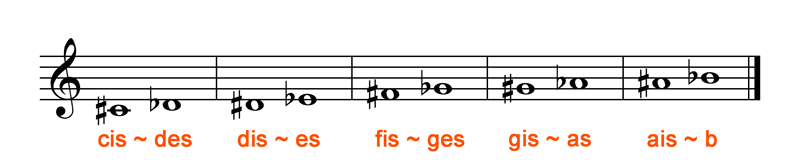
\includegraphics[width=0.7\textwidth]{Bilder/enharmonische-verwechslung.png}
    \caption{Enharmonische Verwechslungen}
\end{figure}
Dieser Unterschied wird das pythagoreische Komma genannt. Die Töne fis und ges wurden später von der gleichstufigen Stimmung gleichgesetzt. Die gleichstufige Stimmung definiert einen Halbtonschritt als 100 Cent, sodass die ganze Oktave gleichstufig verteilt ist und das
pythagoreische Komma aufgelöst wird. Die reine Stimmung basiert, entgegen den anderen beiden Stimmungen, auf den natürlich auftretenden harmonischen Obertönen(\ref{sec:Oberton}) eines Tons. Bei der reinen Stimmung treten noch mehr Probleme mit der Bestimmung der Ganz- und Halbtonschritte auf. Es ergeben sich aus der Definition der reinen Stimmung verschiedene Frequenzverhältnisse. \cite{abcmusik}

\section{Serious Games}
Serious Games sind digitale Spiele, welche nicht nur unterhalten sollen, sondern auch ein weiteres Ziel verfolgen. Dies wird gemacht, um eine Brücke zwischen Bildung und der Vermittlung von neuem Wissen und Unterhaltung zu schlagen. Dieses Ziel wird auch das Characterizing Goal genannt. Dabei ist es wichtig, dass Serious Games dieses zusätzliche Ziel umsetzen wollen, ohne dabei den Spielspaß oder die generelle Spielerfahrung einzuschränken. Die Spiele sollen weiterhin das Hauptziel der Unterhaltung verfolgen und lediglich während dem Spielen automatisch das Characterizing Goal vermitteln. Der Namenszusatz \glqq serious'' soll also nicht bedeuten, dass das Spiel etwa in dem Sinne ernst oder langweilig sind, sondern verweist vielmehr auf die \glqq seriösen'' Branchen in denen Serious Games eingesetzt werden können. Unter diese Branchen fallen unter anderem die Bildung, Sport, Krisenmanagement, Städteplanung, Religion oder Politik \cite{gaiasg} . 
Einige prominente Beispiele sind Spiele, wie etwa \glqq Coding Pirates'' \cite{coding_game}, welches neues Wissen vermitteln möchte, oder ein Spiel welches zur Bewegung anregen möchte, wie etwa \glqq Pokemon Go''\cite{althoff2016influence} oder die \glqq Moto Tiles'' \cite{liu2018playful}. Um Serious Games einheitlich klassifizieren zu können, wurde das sogenannte \glqq Serious Games Metadata Format'' entwickelt. Dieses Format ist aus mehreren Stufen aufgebaut. Die erste Ebene (Core), enthält allgemeine Informationen über das Spiel, welche Interessenten einen Überblick über die Qualität, Innovationen und Anwendungen des Spiel geben sollen. Die zweite Ebene (Detailed) dient Kritikern und Experten als Grundlage der Bewertung eines Serious Games. Sie beinhaltet daher Punkte wie etwa Informationen zur User Experience und einen Fragebogen zur generellen Bewertung. Auf der dritten Ebene (Extension) wird schließlich auf spezifische Aspekte des Spiels eingegangen. So werden hier beispielsweise bei Exergames Trainingsprogramme und genaue Sportübungen bewertet \cite{gobel2011makes}. Eine Plattform, um nach dem Metadaten Format Spiele zu filtern, ist das Serious Games Information Center (SG-IC) \cite{sg_ic}. \\
Das Konzept der Serious Games steht im Gegensatz zu Gamification. Bei der Gamification handelt es sich um den Ansatz, spielerische Komponenten in eine Umgebung einzubinden, welche kein Spiel ist. Ein populäres Beispiele für Gamification ist \glqq Duolingo'' \cite{duolingo}. Spielerische Elemente können ein Highscore System mit online Leaderboard sein oder die Möglichkeit Trophäen zu sammeln. Die Elemente der Gamification sollen dem Nutzer meistens ein Gefühl von Fortschritt geben. 
% TODO add Serious Games kapitel, ganz grob beschreiben

\chapter{Analyse}

%- Wie in der Rechereche vorgegangen (Kontakte, Anhaltspunkte, Wissenschaftler, Suchbegriffe, wichtigste Filter) -> Top Referenzen
%- Studentin befragt nach bestem SotA
%- Was fehlt, was könnte besser sein?
%- Hobby Musiker befragt ob sie soetwas kennen und Interesse hätten, wie wäre es Interessant?
%- Gehörbildungslehrer / Musiklehrer befragen, woran es häufig hakelt und was interessant ist in so einem Programm
%
%
%- tech. Knackpunkt: Wie macht die Game Engine etwas? (Sound Verarbeitung etc.)
%- Auslesen der Mikrofon Daten und direkte Umrechnung mithilfe von gegebenen FFT Methoden in Unity
%- PDA im Rahmen dieser Möglichkeiten
%- Warum keinen komplexeren PDA implementiert ohne eingebaute Unity FFT
Im folgenden Kapitel werde ich zunächst auf den aktuellen Stand der Trainingsprogramme für Gehörbildung eingehen und diese auf ihre wichtigsten Aspekte analysieren. Dabei stelle ich mir auch die Frage, wie man diese noch verbessern könnte. Daraufhin werde ich meinen Recherche- und Analyse-Prozess nach Methoden und Konzepten der Echtzeiterkennung von Audio mit Unity aufzeigen, um diese in einen Prototypen eines Trainingsprogramms einzubinden.

\section{Analyse von Trainingsprogrammen zur Gehörbildung}
%- auf bestimmte Aspekte achten, bei der Analyse
%    - Audio Input?
%    - Arten von Übungen 
%        - Vielfalt
%        - Abdeckung der musikalischen Bereiche (Intervalle, Akkorde, )
%    - Übungsvielfalt
%        - festes Set oder Endlosübungen
%    - Navigierbarkeit
%    -Pädagogisches Konzept
Ich stelle zunächst die interessantesten Anwendungen und Websites zur Gehörbildung vor.
\subsection{Methodik}
%TODO Methodik
%- Auf Pitch Detection achten
%- Übungsarten x 
%- Einführung in Thema  (theorieteil) x
%- Wieder(spielbarkeit) x
%
%- Audio Input?
%    - Arten von Übungen 
%        - Abdeckung der musikalischen Bereiche (Intervalle, Akkorde, )    x
%    - Übungsvielfalt x
%        - festes Set oder Endlosübungen x
%    - Navigierbarkeit x
%    -Pädagogisches Konzept x

% Übung
Ich werde bei der Begutachtung der State of the Art Anwendungen vor allem auf die Aspekte der Übungsvielfalt, sowie auf den Aufbau der Übungen achten. Unter die Übungsvielfalt fällt unter anderem eine Einschätzung der Wiederspielbarkeit und des abgefragten Wissens, sowie die Breite der verfügbaren Übungen zu verschiedenen musikalischen Bereichen innerhalb der Gehörbildung. Zu diesen Bereichen zählen beispielsweise Intervalle, Akkorde, oder Melodiediktate.
% Pädagogisches Konzept
Außerdem möchte ich auf die Weiterbildungsmöglichkeiten und die generelle Wissensvermittlung achten. Unter Wissensvermittlung verstehe ich hier, ob das Wissen beispielsweise innerhalb des Spiels vermittelt wird, oder nur zum Nachlesen bereitgestellt wird. 
% Input + UI
Weiterhin betrachte ich, wie der Nutzer mit der Anwendung interagiert. Dabei sind die Navigierbarkeit, die Eingabemethoden, sowie der generelle Aufbau des UIs interessant. 

\subsection{State of the Art}

Zu den State of the Art Programmen gehören vor allem online Tools zur Unterstützung bei der Gehörbildung. Die folgenden Tools habe ich vor allem durch Befragung von Musikstudenten, sowie durch einfache Suchanfragen gefunden.

\subsection*{Gehörbildungswebsite der staatlichen Hochschule für Musik und darstellenden Kunst Mannheim}
\label{sec:Mannheim}
Hierbei handelt es sich um ein online Tool, bei welchem aus einer festen Anzahl an aufgenommen Hörbeispielen Übungen generiert werden.
Dabei werden die Themen Intervalle, Akkorde, Melodien, Harmonien und Intonation angeboten, wobei die Korrekturmöglichkeit in der Anzeige der Lösungen besteht. Das Lernen der Intervalle ist so strukturiert, dass der Nutzer Töne vorgegeben bekommt
und die Intervalle zwischen den Tönen bzw. zu einem Grundton bestimmen soll. Die Website überprüft dabei nicht selbst, ob der Nutzer die Aufgabe richtig absolviert hat, der Nutzer muss sich selbst überprüfen. 
Es gibt mehrere Arten von Intervalltraining: so kann man seine Fähigkeiten in diatonischen Stufen, also innerhalb einer Tonleiter ohne Halbtöne, oder durch das Erkennen von reinen Intervallen zwischen den einzelnen Tönen, verbessern. Es gibt weiterhin die Möglichkeit in ganzen Tonreihen
direkte und indirekt erklingende Intervalle zu erhören bzw. wahrzunehmen. Man erhält zugriff auf die Übungen, nachdem man einen kostenlosen Account 
erstellt hat. Die Übungen sind unterteilt in einzelne Reiter in die einzelnen Lektionen. Es existiert ein kurzer einleitender Text, welcher den Nutzen der Website kurz erläutert und eine schnelle Erklärung, wie vorzugehen ist beim Lernen. Es werden keine Module oder Lektionen angeboten, welche die Grundlagen der Aufgaben näher erläutern.\\
Die Website bietet allerdings nur die Aufgaben an, das heißt es gibt keine eingebaute Überprüfung, weder als Texteingabe noch als Audioinput vom Nutzer. \cite{hfmdk_mannheim}

\subsection*{Musictheory.net und Tenuto}
\label{sec:Musictheory.net} \label{sec:Tenuto}
Die Website Musictheory bietet eine Vielzahl von Übungen in verschiedenen Disziplinen an. Es existieren theoretische Lektionen, welche das fundamentale Wissen herstellen sollen, sowie Übungen, um dieses abzufragen und zu testen. 
Die Lektionen umfassen die Grundlagen der Musik, wie etwa die verschiedenen Notenschlüssel oder das Notenlesen, bis hin zu verschiedenen Arten von Akkorden und wie diese aufgebaut werden. Die Übungen umfassen dementsprechend ein ähnlichen Wissensumfang, es wird beispielsweise das Notenlesen abgefragt oder die Tonart, aber man kann auch Gehörbildung üben, wo man das Erkennen von Tönen bis hin zu Akkorden üben kann. Bei diesen Übungen kann man
allerdings nur das gehörte aus einer Liste auswählen. Ein Unterschied zu der Website der HfMdK Mannheim besteht darin, dass Musictheory.net Antwortmöglichkeiten gibt und bei diesen ein Feedback gibt, ob 
die Antwort richtig war. Auch hier gibt es kein Feature, welches gesungene Intervalle überprüft. Musictheory.net hat eine App für iOS entwickelt, welche die Aufgaben, die auch auf der Website zur Verfügung stehen,
mit erweiterten Funktionen bereitstellt. Die Funktionen der App umfassen zusätzlich zu den Aufgaben der Website eine Möglichkeit, Aufgabentypen anzupassen, um diese so spezifisch zu lernen. Des weiteren wurde ein Challenge Modus in der App hinzugefügt, welcher den Nutzer herausfordert, unter Zeitdruck Aufgaben richtig zu beantworten und den Highscore zu verbessern. Das User Interface der App wird auf der Webseite als einfach zu bedienen beworben und bietet eine klare Benutzererfahrung . 
Die App kostet 3.99\$, wohingegen die Website kostenfrei ist und ohne Benutzerkonto verwendet werden kann. Es ist noch anzumerken, dass sowohl die Website, als auch die App nur auf Englisch verfügbar sind, was eine sprachliche Barriere für den Nutzer darstellen kann. Es kann außerdem zu missverständnissen kommen, da z.B das H im Deutschen ein B im Englischen ist. \cite{musictheory}

\subsection*{Teoria}
\label{sec:Teoria}
Teoria bietet ähnlich wie Musictheory, einen Theorieteil und einen Praxisteil an. Im Theorieteil werden auch hier die Grundlagen der Musik vermittelt, wie beispielsweise das Notenlesen oder was ein Intervall ist und wie diese aufgebaut werden.
Im praktischen Teil ermöglicht Teoria es dem Nutzer, seine eigenen Aufgaben selbst zu gestalten, indem man die abzufragenden Intervalle oder auch den Grundton einstellen kann. Es ist außerdem möglich, das sogenannte vom Blatt Singen zu trainieren, was nichts anderes
heißt, als direkt die Noten und den Rhythmus richtig zu singen, ohne es vorher gehört oder geübt zu haben. Das Singen wird allerdings auch hier nicht überprüft, es ist nur ein Angebot gegeben, sich selbst überprüfen zu können. Es werden weiterhin Übungsangebote in den
Aufgabenbereichen der Intervalle, Akkorde, des Rhythmus und der Tonarterkennung angeboten. Die Aufgaben werden durch die vom Nutzer voreingestellten Parameter zufällig generiert und können somit auch an die Bedürfnisse des Nutzer angepasst werden. Die Website hat ein relativ einfaches und intuitives Design, ist allerdings nur auf Englisch verfügbar, was beispielsweise die Namen der Akkorde betrifft und durchaus eine Umstellung für den Nutzer darstellen kann. \cite{teoria}

\subsection*{JKG Neigungskurs Musik}
\label{sec:Neigungskurs}
Die Website des Justus-Knecht-Gymnasium Bruchsaal bietet ein kleines vordefiniertes Set an Aufgaben, für die Vorbereitung auf die Musik Abiturprüfung, an. Zu den Aufgabentypen zählen Rhythmusdiktate, Melodiediktate, sowie das Erkennen von Intervallen und Akkorden.
Wie bereits erwähnt sind die Aufgaben vordefiniert und bieten keinerlei Möglichkeit sie nach den Bedürfnissen des Nutzers anzupassen. Die Aufgaben bilden eine grobe Übersicht über die möglichen Aufgabentypen und dienen nur als Lernhilfe oder zur Überprüfung; sie sind jedoch nicht geeignet als alleiniges Lernmittel oder zur täglichen Festigung der Fähigkeiten. Es existiert dementsprechend auch keine Schrittweise Einführung in die Grundlagen der Musik oder der Gehörbildung. Des Weiteren ist die Bedienbarkeit und Nutzerfreundlichkeit der Website mangelhaft, da die Soundbeispiele über Soundcloud zwar in die Website eingebunden sind, die Lösungen jedoch nur in 
PDFs zu finden sind, welche zunächst heruntergeladen werden müssen. \cite{jkg_bruch}

\subsection*{Musikgrad}
\label{sec:Musikgrad}
Musikgrad bietet einige simple Aufgabentypen und Trainingsmethoden zu Intervallbestimmung, aber auch zu der Bestimmung von Akkorden und den Grundlagen der Musik, wie etwa das Notenlesen. Die Theorieaufgaben bzw. Lektionen sind dabei in Lektionen und Module innerhalb einer Lektion strukturiert, welche das Thema so Schritt für Schritt näher erläutern. Da einige Aufgaben allerdings leider Flash Player benötigen, sind diese nicht mehr zugänglich. Ich beschränke mich im Folgenden nur auf die verfügbaren Aufgaben, welche allerdings immer noch die wichtigsten Funktionen abdecken. Es wird die Möglichkeit geboten, Intervalle zu erhören; es werden dabei zwei Töne gleichzeitig abgespielt und der Nutzer muss aus allen Intervallen entscheiden, welches erklungen ist. Es wird dabei die Möglichkeit gegeben, die abzufragenden Intervalle zu konfigurieren, um so auf eigene Schwächen genauer einzugehen. Es gab offensichtlich mal die Möglichkeit, auch zu einem gegebenen Grundton ein Intervall in einem Notensystem zu vervollständigen, diese Funktion
ist allerdings mittlerweile veraltet und nicht mehr verfügbar. Auch bei Musikgrad gibt es keine Möglichkeit für den Nutzer, Intervalle zu singen und durch die Website überprüfen zu lassen. Die Website an sich ist simpel aufgebaut, sodass man durch eine einfache Auswahl zu den verschiedenen Übungen kommt. Die Übungen sind innerhalb einer eingebundenen Anwendung im Browser verfügbar, sodass kein Vollbildmodus verfügbar ist. \cite{musikgrad}


\subsection*{Earbeater}
\label{sec:Earbeater}
Earbeater ist ebenfalls ein Onlinetool, welches mehrere Übungsangebote spannend von Intervallbezeichnung bis hin zu der Identifizierung von Tonleitern einbindet. Die Aufgabentypen sind hierbei nochmals in Unterkategorien eingeteilt, welche verschiedene Bereiche der 
Oberkategorie abdecken. Bei Intervallen handelt es sich hier beispielsweise um verschiedene Kombinationen von Intervallarten, welche aufsteigend oder absteigend abgefragt werden können. Es werden in jeder Aufgabe kurz die relevanten Schlüsselwörter erklärt, sodass der Nutzer das nötige Wissen hat, um die Aufgabe zu bearbeiten. Es ist dem Nutzer möglich, die Intervalle unter mehreren Auswahlmöglichkeiten zu wählen, eine andere Eingabe der Lösung ist jedoch nicht möglich. Eine Tonerkennung ist also auch hier nicht vorhanden. Die Website bietet die Möglichkeit an ein Benutzerprofil zu erstellen, um die Fortschritte und Highscores der Aufgaben zu speichern. Es ist außerdem möglich eigene Aufgaben zu erstellen und diese 
auch mit anderen Nutzern zu teilen. Earbeater ist ebenfalls wie Teoria nur auf Englisch verfügbar. Die Website besticht mit einem modernen und übersichtlichem Design, welches sowohl für eine einfache Handhabung sorgt, als auch für eine übersichtliche Darstellung der Ergebnisse der Übungen. Earbeater bietet außerdem 
eine iOS Anwendung an, sodass die Nutzer auch von Unterwegs üben können. \cite{earbeater}

\subsection*{Tonedear}
\label{sec:Tonedear}
Tonedear bietet wie die meisten anderen Tool mehrere Aufgabentypen, sowie die Möglichkeit diese zu konfigurieren. Es werden allerdings keine vorgefertigten Kurse angeboten; es gibt also nur zufällig generierte Aufgaben, welche keinen aufbauenden Lehrinhalt vermitteln. Dieses Defizit kann Tonedear dafür mit der Möglichkeit der Erstellung von Lehreraccounts ausgleichen. Ein Lehrer kann somit für seine Klasse eigene Aufgaben erstellen und somit auch einen Lehrplan verfolgen. Zu den Funktionen des Lehreraccounts zählen außerdem die Möglichkeiten die Abgaben der Schüler einzusehen und die Klassenliste zu verwalten. Es ist dem Nutzer auch hier die Möglichkeit gegeben, die eigenen Aufgaben
zu einem gewissen Maß zu konfigurieren, wie zum Beispiel durch die Auswahl aus drei verschiedenen Aufgabensets bei den Intervallaufgaben. Eine Mikrofonunterstützung wird auch von Tonedear nicht angeboten. Die Website ist einfach aufgebaut und bietet eine simple Navigation zu den einzelnen Aufgaben. 
Das Konfigurieren der Aufgaben ist ebenfalls intuitiv. \cite{tonedear}


\subsection*{Earmaster}
\label{sec:Earmaster}
Earmaster ist eine professionell entwickelte Gehörbildungssoftware, welche von dem gleichnamigen Unternehmen entwickelt wird. Earmaster existiert seit den 1990er Jahren und wird seitdem immer weiterentwickelt und deckt somit einen Großteil der Bedürfnisse der Nutzer ab. Die Software kann online für
4\$ im Monat gekauft werden und bietet neben kapitelweise aufgebauten Modulen auch die Möglichkeit,benutzerdefinierte Übungen zu generieren. Die Funktionen umfassen eine modulweise Einführung in die Gehörbildung, wobei Themenbereiche von der Tonhöhe bis hin zu Akkordfortschreitungen abgedeckt werden. Weiterhin bietet Earmaster neben diesem sogenannten Einsteigerkurs auch Workshops, welche das erlangte Wissen aus dem Einsteigerkurs weiter festigen sollen. Diese Workshops gehen dabei auch Modulweise vor und fragen dabei die gewünschten Inhalte gezielter ab. Betrachtet man hierbei beispielsweise den \glqq Intervall-Singen'' Workshop, so werden dort einzelne Herangehensweisen des Intervallsingens behandelt und abgefragt. Die Software bietet für ihre zahlreichen verschiedenen Aufgabentypen eine Vielfalt an Arten der Eingabe der Lösungen. Es ist möglich Intervalle selbst zu singen, Töne einzeln auf das Notensystem zu platzieren, sowie aus einer Auswahl an Antworten zu wählen. Die Tonerkennung ist konfigurierbar, es werden dem Nutzer mehrere Tonlagen zur Auswahl gestellt, sowie die Möglichkeit gegeben seine eigene Tonlage zu definieren. Weiterhin werden nicht nur die tatsächlichen Tonhöhen als richtige Antwort gewertet, sondern auch die jeweiligen Oktaven des gesungenen Tons, sodass der Nutzer immer in der angenehmsten Tonlage singen kann. Außerdem gibt es extra einige Jazz Workshops, welche die besonderen Eigenschaften der Akkorde und Akkordfolgen der Jazzmusik behandeln. Der Nutzer kann zudem seine bereits vollendeten Lektionen
in einer Statistik einsehen, wobei dort auch der Gesamtfortschritt der Übungen eingesehen werden kann. Bei dem Absolvieren der Übungen selbst bekommt der Nutzer direktes Feedback in Form von 5 möglichen zu erreichenden Sternen, welche je nach Genauigkeit und Intonation des Tons vergeben werden. Weitere Gamification Elemente, wie etwa eine das Aufzeichnen einer Übungsstreak, welche angibt wie viele Tage man täglich geübt hat, gibt es nicht. \cite{earmaster}

\subsection{Analyse der relevantesten Anwendungen}

%- Auf Pitch Detection achten
%- Übungsarten x 
%- Einführung in Thema  (theorieteil) x
%- Wieder(spielbarkeit) x
%
%- Audio Input?
%    - Arten von Übungen 
%        - Abdeckung der musikalischen Bereiche (Intervalle, Akkorde, )    x
%    - Übungsvielfalt x
%        - festes Set oder Endlosübungen x
%    - Navigierbarkeit x
%    -Pädagogisches Konzept x
%TODO Methodik FElder aufschlüsseln in unterkapitel

Im Folgenden möchte ich die oben genannten Anwendungen zu Gehörbildung unter bestimmten Gesichtspunkten vergleichen und analysieren, um so auf die Stärken und Schwächen dieser schließen zu können. Die wichtigsten Gesichtspunkte sind dabei die Übungsvielfalt, ob die Übungen und wie gut sie erläutert werden  und außerdem die Nutzbarkeit der Anwendung. Unter die Nutzbarkeit fallen Punkte wie etwa die Übersichtlichkeit der Anwendung, die Vielfalt der Eingabemethoden und inwiefern dem Nutzer Feedback zu der Aufgabe gegeben wird. Weitere Aspekte sind Anreize kontinuierlich zu Üben, sowie, wenn vorhanden, die Genauigkeit der Tonerkennung. Ich erhoffe mir mit den Ergebnissen dieser Analyse auf die wichtigsten Merkmale einer Gehörbildungsanwendung schließen zu können und wie man eine solche optimieren kann. \\\\

Alle Anwendungen haben gemeinsam, dass sie mehrere Aufgabentypen zu Intervallen, Akkorden und Tonhöhe abfragen können. Diese Aufgabenbereiche sind zentrales Thema der Gehörbildung und dementsprechend wichtig und vielfältig umgesetzt. 
Die Umsetzung der Aufgaben jedoch weicht stark unter den bekanntesten Programmen ab. So ermöglichen die Webseiten der HfMdK Mannheim und des JKG Neigungskurses nur das beantworten von vordefinierten Aufgaben, wohingegen der Rest entweder zufällig generierte Aufgaben abfragt oder anpassbare Aufgaben generiert.
Einer der Unterschiede in diesem Zusammenhang ist auch, dass vordefinierte Aufgaben aufeinander aufbauen können oder eine gewisse interne Lernstruktur verfolgen können, welche beispielsweise stetig den Schwierigkeitsgrad erhöht. Weiterhin können vordefinierte Aufgaben den Bezug zur echten Musik besser herstellen. So können mehr Aufgaben zu Intervallen und Akkorden gestellt werden, welche auch in der Musik häufiger vorkommen. Allerdings lässt sich durch zufällig generierte Aufgaben eine größere Vielfalt an Aufgaben gewährleisten, was den Nutzer mehr dazu anregt täglich zu üben. Ein idealer Ansatz wäre hier also einige vordefinierte, bestenfalls von professionellen Musiklehrern entwickelte Aufgaben zur Verfügung zu stellen, aber auch die Möglichkeit zu bieten, durch konfigurierbare Endlosübungen dieses Wissen zu festigen, wie es Earmaster  oder Earbeater anbieten. Im Zusammenhang mit der Übungsvielfalt steht natürlich auch die Abdeckung der Teilbereiche der Gehörbildung. Bestenfalls bietet eine Anwendung einen kompletten Überblick über alle relevanten Themen und bietet zu diesen auch Übungen an. In der Realität setzen das auch die meisten Übungsangebote durch. So bietet die Website des Musik Neigungskurses der JKG Bruchsaal zwar nur vordefinierte Aufgaben an, dafür aber in dem Großteil der relevanten Themengebiete. Tatsächlich bietet jedes der oben genannten Trainingsprogramme die Möglichkeit, eine Vielzahl an verschiedenen Übungsarten zu absolvieren.  \\
Soll das Trainingsprogramm allerdings nicht nur für bereits ausgebildete Musik zugänglich sein, so benötigt dieses auch theoretische Teile, welche mit den praktischen Übungen Hand in Hand gehen, um neuen Musikern diese Konzepte möglichst verständlich zu vermitteln. Diese Einführung in Themen setzen alle der oben genannten Programme um, indem sie Zugriff auf theoretische Sachtexte bieten, welche
die Musiktheorie hinter den Konzepten erklären oder die theoretischen Teile zusammen mit praktischen Übungen erklären, wie es etwa bei Earmaster der Fall ist. Jedoch hat der Großteil der Trainingsprogramme nur ein rudimentäres Angebot an theoretischer Weiterbildung, was meiner Meinung nach eins der größten Probleme bei diesen Trainingsprogrammen ist. Die theoretischen 
Übungen bzw. Texte können nicht nur für einen Anfänger hilfreich sein, sich neues Wissen anzueignen, sondern auch für erfahrenen Musiker, welche vielleicht nur eine Auffrischung der theoretischen Inhalte benötigen. Ein weiterer großer Kritikpunkt an den oben genannten Programmen ist, dass nur minimal Elemente der Gamification implementiert wurden. So implementiert Earmaster ein Feedback System, 
welches dem Nutzer, nach einer abgeschlossenen Aufgabe, zwischen einem und fünf Sternen verteilt. Die verteilten Sterne werden allerdings nicht in einer Statistik festgehalten, oder in einem online Leaderboard mit Freunden oder anderen Nutzern verglichen. Die restlichen Anwendungen setzen in dieser Hinsicht gar kein Gamification Element um. Ich sehe hier bei allen Anwendungen großes verschenktes Potential und denke ein solches System würde dem Nutzer einen viel größeren Anreiz geben sich weiterbilden zu wollen. Tatsächlich wird bei allen Anwendungen die intrinsische Motivation des Nutzer vorausgesetzt, dass dieser sich fortbilden möchte. \\ 
Wichtig ist außerdem die Bedienbarkeit der Anwendungen. Die meisten Anwendungen ermöglichen es dem Nutzer mithilfe von mehreren Button unter einem Notensystem ihre Eingabe zu machen. Dieses Design ist einfach und übersichtlich, jedoch reizt es meiner Meinung nach nicht sämtliche Möglichkeiten der Wissensvermittlung aus. Dem Nutzer kann zusätzlich zu dem Ablesen aus dem Notensystem und dem anschließenden Beantworten der Frage durch einen Knopfdruck das Verwenden und Lesen eines Notensystem beigebracht werden, indem man beispielsweise eine Eingabe durch das klicken in ein Notensystem ermöglicht. Diese Art der Eingabe wird von manchen der Anwendungen umgesetzt, wie etwa Musictheory oder Earmaster. \\
Eine weitere Eingabemethode im Zusammenhang mit Noten ist das Erkennen von gesungenen oder anders erzeugten Tönen vom Nutzer. Eine solche echtzeit Erkennung von erklingenden Noten setzt bis auf Earmaster keins der oben genannten Programme um. Earmaster ermöglicht es \glqq blind'' zu singen, das heißt, ohne dass der Nutzer seinen aktuell gesungenen Ton live überprüfen kann. Hat der Nutzer die 
Note lang genug gehalten, so wird Feedback gegeben mithilfe einer Linie durch das Notensystem, welche den Verlauf des gesungenen Tons angibt. Ich halte dieses Feature für eines der wichtigsten in allen oben genannten Anwendungen, da es bei dem Nutzer nicht nur Wissen abfragt, sondern auch aktiv die musikalischen Fähigkeiten trainiert.
Eine weitere gute Eingabemethode, welche von einigen der genannten Anwendungen umgesetzt wird, ist die Eingabe der Töne mit einer virtuellen Klaviatur. Diese Art der Eingabe macht vor allem für solche Nutzer Sinn, welche bereits vertraut mit dem Klavier sind und so die Verbindung von Gelerntem direkt auf ihr Instrument übertragen können. Für 
Anfänger ist diese Eingabemethode offensichtlich nicht geeignet, da diese häufig nicht über das Wissen verfügen, wo welche Töne auf einer Klaviatur sind. \\\\
Zusammenfassend lässt sich sagen, dass viele der Anwendungen offenbar als simple Unterstützungen beim Lernen gedacht sind. Sie sind dementsprechend nicht für die breite Öffentlichkeit entwickelt worden, sondern zum Großteil für Musikstudenten oder Schüler mit Leistungsfach Musik, die einzige Ausnahme bildet augenscheinlich Earmaster, was so umfangreich ist mit so vielen verschiedenen Modulen zum Lernen und einer sehr großen Anpassungsmöglichkeit an die einzelnen Bedürfnisse der Nutzer, dass es sämtliche anderen Programme übertrifft und somit den aktuellen Stand der Trainingsprogramme am besten widerspiegelt. 

\section{Analyse von Methoden und Konzepten zur Echtzeiterkennung und Verarbeitung von Audio Input vom Anwender mit Unity}
%- Echtzeit Audio einlesen
%- Auf Audio zugreifen (GetSpectrumData, GetData, mehrere Ansätze -> Ringbuffer, direkte Verarbeitung)
%- PDA - Pitch Detection Algorithm (WElche Methoden gibt es warum für was entschieden)
%- Genauigkeit verbessern (Noise Filter, Threshold, Interpolation)
%- Noise Filter welche ansätze gibt es, warum für einfache Avg Lösung entschieden
%- Threshold für Ausschläge geben
%- Interpolation warum Newton und warum nur 3 Punkte
Ich gehe zunächst auf den Rechercheprozess zu den Ansätzen der Echtzeiterkennung von gesungenen Tönen ein und will daraufhin die interessantesten Ansätze analysieren. 

\subsection{Recherche}

Ich bin bei der Recherche schrittweise vorgegangen und habe zunächst nach der Tonverarbeitung und Aufnahme in Unity recherchiert. Ich habe zunächst in der Unity Dokumentation nach den Schlagworten Audio, Sound, Frequency und Microphone gesucht. Unter dem Schlagwort Microphone bin ich auf die Dokumentation der Microphone Klasse gestoßen, wo mir schließlich auffiel, dass es keinen direkten Weg gibt, um in Echtzeit auf die Microphone Daten zuzugreifen. \cite{unity_doku_micro} Da ich zunächst herausfinden wollte, wie und ob es möglich ist das Mikrofon in Echtzeit auszulesen mit Unity recherchierte ich weiter. Nach einer Suchanfrage \glqq Unity Microphone in realtime'' bin ich auf einen Artikel aus den Unity Foren gestoßen, welcher genau das Problem behandelte. \cite{unity_forum_realtime} Jedoch ergaben sich nach ersten Tests Probleme mit der Latenz, da diese noch nicht auf Echtzeit-Niveau war. Meine Recherche führte mich nun wieder zurück in die Unity Dokumentation wo ich nach weiteren Suchanfragen zu Audio auf den AudioManager stieß. In den Projekteinstellungen lässt sich die DSP Buffer Size der Anwendung anpassen zwischen bester Latenz und bester Qualität. \cite{unity_doku_audioManager} Veränderte ich diese Einstellung auf \glqq good Latency'' funktionierte der kleine Test zum Einlesen der Daten in Echtzeit. Unter den Ergebnissen der oben genannten Schlagworten in der Unity Dokumentation fand ich als nächstes eine Übersicht zu Audio in Unity. \cite{unity_doku_audio} Diese Übersicht leitete mich weiter zu detaillierteren Artikeln zu Audio Verarbeitung in Unity. Zu diesen Artikeln gehörten Audio Source, Audio Listener, Audio Mixer, Audio Effects und Reverb Zones, wobei sich die Reverb Zone nach kürzerer Recherche als irrelevant herausstellte. Die restlichen Artikel waren hingegen von Nutzen für mein weiteres Vorgehen. Die wichtigste Information habe ich aus der Scripting Dokumentation der Audio Source erhalten. Die Audio Source besitzt in der Scripting API eine statische Methode, welche es mir ermöglicht das Spektrum der Audiodaten des dazugehörigen AudioClips zuzugreifen bzw. es zu berechnen. \cite{unity_doku_spectrumData}
Die Funktion ermöglicht es direkt das Spektrum des AudioClips einer AudioSource mithilfe einer schnellen Fouriertransformation zu berechnen. Ich habe mich nun also mehr mit den mir zur Verfügung stehenden schnellen Fouriertransformationen von Unity befasst. Zu den von Unity bereitgestellten Fensterfunktionen zählen Rectangular, Triangle, Hamming, Hanning, Blackman und BlackmanHarris. 
\\ % TODO keine Stories erzählen ! Nur die gewählten recherchemethoden und ergebnisse vorstellen
Ich habe nun mit der Fouriertransformation einige Ansätze ausgetestet, ob und wie gut sich aus einer einfachen Fouriertransformation der erklingende Ton herausfiltern lässt. Ein naiver Ansatz war zunächst das absolute Maximum der Fouriertransformation zu wählen und diesen als erkannten Ton weiter zu verarbeiten. Dieser Ansatz funktionierte zunächst sehr gut mit Sinuswellen förmigen Tönen. Als ich anfing die Erkennung mit meiner eigenen Stimme zu testen, wurde mir jedoch schnell klar, dass die Obertöne (\ref{sec:Oberton}) der menschlichen Stimme einen komplexeren Ansatz der Tonerkennung benötigen würde. Ich setzte mich als nächstes also mit einigen Pitch Detection Algorithmen (PDA) bzw. Ansätzen auseinander. Ich fand unter den Suchbegriffen \glqq Pitch detection algorithm'' bei Google Scholar und Google einige PDAs. Dabei achtete ich schon hier darauf, dass diese einerseits eine gute Erkennungsrate haben würde, sodass ich auf Basis dessen ein Trainingsprogramm aufbauen kann, jedoch nicht zu viel Rechenarbeit benötigen würden. Weitere Aspekte bei der Auswahl eines Algorithmus waren, wie umsetzbar dieser mit den von Unity gegebenen Ressourcen ist. Die Ansätze, welche ich als interessant erachtete, stelle ich im nächsten Abschnitt vor. 


\subsection{Audioinput und Verarbeitung mit Unity}
Bevor wir uns mit der eigentlichen Erkennung von Tönen beschäftigen können, muss etabliert werden, wie Töne vom Nutzer mithilfe von Unity eingelesen und gespeichert werden. Glücklicherweise bietet Unity einige Hilfen um Audio einzulesen. Es ist möglich auf Audiorohdaten vom Nutzer zuzugreifen und somit mit diesen zu arbeiten. Weiterhin ist es auch möglich das Frequenzspektrum dieser Audiodaten, mithilfe einer von Unity bereitgestellten Methode, zu berechnen. Möchte man jedoch diese Methode verwenden, so ist man auch an die Datenstrukturen von Unity gebunden. Die Möglichkeiten umfassen jetzt, entweder eine eigene Datenstruktur entwickeln zu können oder das Frequenzspektrum mithilfe der internen Methoden zu berechnen. Wie man in der nächsten Sektion erkennen wird, bietet eine eigene Datenstruktur eine größere Auswahl an Pitch Detection Algorithmen, da durch die eigene Datenstruktur mehr potentielle Informationen zur Verfügung stehen. Es ist somit möglich, mithilfe von eigens implementierten schnellen Fouriertransformation selbst das Frequenzspektrum der Daten zu berechnen. Auf der anderen Seite ist es wahrscheinlich, dass die von Unity zur Verfügung gestellten Funktionen im Kontext einer Unityanwendung performanter sind. Weiterhin ist bereits bekannt, dass der Grundton eines Klangs immer die tiefste dominante Schwingung im Frequenzspektrum des Klangs ist. Aus diesem Vorwissen, können wir schließen, dass eine Fouriertransformation auf den Audiodaten des Nutzers sehr wichtig sein wird. Mit dem Hintergrund, eine echtzeit Tonerkennung entwickeln zu wollen, fällt dementsprechend die Auswahl, um Audioinput vom Nutzer zu lesen und weiterzuverarbeiten auf die Funktion von Unity. 

\subsection{Ansätze der Pitch Detection Algorithmen}
Infrage kommende Pitch Detection Algorithmen lassen sich in zwei Klassen einteilen. Es gibt zum einen Algorithmen, welche versuchen den Grundton zu berechnen, indem Operationen auf dem zeitabhängigen Signal ausgeführt werden. So kann beispielsweise der Grundton berechnet werden, indem man sich wiederholende Frequenzmuster sucht und aus diesen auf den Grundton schließt. \cite{cuadra2001hps}
Die andere Klasse versucht hingegen, den Grundton aus dem Frequenzspektrum zu berechnen. Wir wissen bereits, dass der Grundton innerhalb eines Spektrums die tiefste schwingende Frequenz in diesem ist. Es gibt innerhalb dessen verschiedene Ansätze diese tiefste Frequenz zu berechnen, wie es etwa das sogenannte Cepstrum macht, welches zunächst das Frequenzspektrum berechnet, innerhalb diesem dann alle Werte logarithmiert und schließlich wieder die Umkehrfunktion der Fouriertransformation anwendet. Auf die Vorteile und Nachteile dieser Ansätze und auf weitere Unterschiede innerhalb dieser möchte ich nun eingehen. \\
Ich fange zunächst mit den Algorithmen an, welche nicht innerhalb des Frequenzspektrum arbeiten. Unter diesen Ansatz fallen Algorithmen und Ansätze wie etwa die \glqq zero-crossing rate'', \glqq average magnitude difference function (AMDF)'' oder die \glqq average squared mean difference function (ASMDF)''. Ich möchte einen kurzen Überblick über die Funktionsweisen dieser Algorithmen geben.

\subsubsection*{Zero-crossing Rate (ZCR)}
Die ZCR ist einer der einfachsten Techniken, um die Grundfrequenz innerhalb eines Klangs zu berechnen. Es wird, wie der Name schon verrät, gezählt, wie oft das Signal vom Positiven auf Null und weiter ins Negative fällt oder anders herum vom negativen Raum auf Null und in den positiven Raum ansteigt. Man kann aus der Häufigkeit dieser crossings die Grundfrequenz nun wie folgt berechnen. 
$$ F_{Signal} = \frac{zcr * f_{Sample}}{2 * |f_{Sample}|}$$
Wobei $f_{Sample}$ die Samplerate der Aufnahme ist, $|f_{Sample}|$ die Anzahl der untersuchten Samples und $zcr$ die erkannten zero-crossings. Jedoch ist dieser Ansatz in den meisten Fällen sehr ungenau und funktioniert nur gut bei Sinustönen. Die Laufzeit des Algorithmus ist hingegen sehr gut aufgrund seiner sehr simplen Natur. \cite{amado2008pitch}

\subsubsection*{Average magnitude difference function (AMDF)}
Der AMDF versucht den Unterschied zwischen dem Originalsignal und einer verzögerten Version des gleichen Signals zu minimieren. Es wird dabei so vorgegangen, dass das verzögerte Signal von dem Original subtrahiert wird und anschließend die Größen der Unterschiede summiert werden. Minimiert man den berechneten AMDF Wert, so erhält man eine ungefähre Näherung an die Grundfrequenz. \cite{ross1974average} Die mathematische Definition lautet wie folgt.
$$ D_r = \frac{1}{L} \sum_{j=1}^L |S_j - S_{j-r}| $$
$r$ beschreibt hierbei die Verzögerung des Signals. Der Algorithmus kann je nach Größe des Verzögerungsfensters eine große Rechenzeit beanspruchen. Der Unterschied zwischen dem AMDF und dem average squared mean difference function (ASMDF) liegt lediglich darin, dass bei letzterem die Differenzen zwischen den Signalen zusätzlich quadriert werden. Diese Anpassung führt zu einer höheren Robustheit
\\\\
Es existieren weiterhin Algorithmen, welche nicht auf dem ursprünglichen Zeitabhängigen Signal arbeiten, sondern auf dem frequenzabhängigen Signal, dem Spektrum. Zu diesen Algorithmen zählen die sogenannten \glqq Cepstrum Analyse'', sowie das \glqq harmonic product spectrum'' und ein \glqq Maximum Likelihood'' Ansatz. All diese Methoden setzen voraus, dass mindestens eine Fouriertransformation auf dem Signal durchgeführt wird.

\subsubsection*{Cepstrum}
Das Cepstrum beschreibt ein Signal, welches zunächst mit Hilfe einer Fouriertransformation in den Frequenzraum überführt wird. Daraufhin wird innerhalb des Frequenzraums logarithmiert und schließlich wieder die Umkehrfunktion der Fouriertransformation angewandt. Welche Bestandteile im zweiten Schritt genau logarithmiert wird, hängt von der Art des Cepstrums ab. Wendet man das \glqq Power Cepstrum'' an, so wird das \glqq Power Spectrum'' logarithmiert. Um das \glqq Complex Cepstrum'' zu berechnen, wird das gesamte Frequenzspektrum logarithmiert und möchte man das \glqq Real Cepstrum'' berechnen, so muss man die Amplitudenwerte logarithmieren.  \cite{oppenheim2004frequency} Zur Pitch Detection ist jedoch nur das Complex Cepstrum geeignet. Möchte man aus diesem nun die erkannte Grundfrequenz berechnen, so muss man lediglich das absolute Maximum wählen. 

\subsubsection*{Harmonic product spectrum}
Ein weiterer Ansatz, um die Grundfrequenz zu berechnen besteht darin, den größte gemeinsamen Teiler der Obertöne zu berechnen. Wie wir bereits wissen, sind die Obertöne nichts anderes als Vielfache der Grundfrequenz. So sind beispielsweise für eine Grundfrequenz von 220Hz einige Obertöne 440Hz, 660Hz und 880Hz. Es ist trivial, dass der größte gemeinsame Teiler von diesen Werten 220Hz ist, was wieder der Grundfrequenz entspricht. Das Harmonic product spectrum nutzt diesen Sachverhalt aus, indem es das Spektrum um immer steigende Faktoren $1,2,3,...,N$ downsampled bzw. anschaulich erklärt staucht. Legt man die gestauchten Spektren übereinander, so muss die Grundfrequenz auf dem gleichen Wert liegen, wie der jeweils $1,2,3,...,N$ Oberton. Multipliziert man diese Spektren dementsprechend miteinander, so ist der größte Ausschlag bei der Grundfrequenz zu finden. Bei diesem Ansatz kommt es häufig zu Oktavenfehlern, sodass der Ton eine Oktave zu hoch erkannt wird. \cite{cuadra2001hps}
\begin{figure}[H]
    \centering
    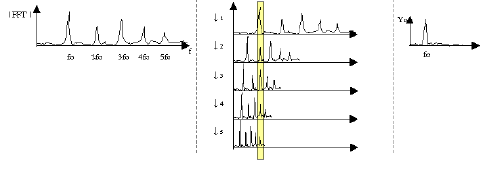
\includegraphics[width=1\textwidth]{Bilder/hps_algo.png}
    \caption{Überblick über den HPS Algorithmus \cite{cuadra2001hps}}
    \label{sec:hps_algo}
\end{figure}

\subsubsection*{Maximum Likelihood}
Der Maximum Likelihood Algorithmus versucht das vorhandene Spektrum mit einer Menge an idealen Spektren zu vergleichen und wählt anhand dieser den Ton aus, der diesem am meisten ähnelt. Dabei versucht der Algorithmus den Fehler zwischen dem gegebenen Spektrum und den idealen Spektren zu minimieren. Da dieser Algorithmus fest definierte Referenzspektren benötigt, funktioniert er am besten, wenn der Ton von einem Instrument erzeugt wird, welches eine feste Stimmung hat, wie beispielsweise ein Klavier. Andernfalls kann es zu stark springenden Ergebnissen kommen. \cite{cuadra2001hps}

\subsection{Analyse der algorithmischen Ansätze zur Pitch Detection}
\label{sec:analyse_echtzeit}
In der folgenden Analyse will ich sowohl die Komplexität der Algorithmen berücksichtigen, als auch die erwartete Robustheit. Ziel der Analyse soll sein, die Ansätze der Algorithmen aufzubereiten, um daraufhin einen Algorithmus zu konzipieren, welcher für eine Umsetzung in Unity geeignet ist. \\
Das größte Unterscheidungsmerkmal der oben vorgestellten Algorithmen ist die Notwendigkeit einer Fouriertransformation. Das Berechnen der Fouriertransformation fügt einen weiteren rechenintensiven Schritt zu dem Algorithmus hinzu. Bei der Entwicklung eines Algorithmus, welcher Ergebnisse in Echtzeit liefern muss, ist das offensichtlich ein negativer Punkt, welcher zu berücksichtigen ist. Naiv betrachtet sollten die Algorithmen, welche im Frequenzbereich arbeiten auch rechenintensiver sein. So benötigt das Cepstrum eine Fouriertransformation und zusätzlich die Umkehrfunktion dieser. Das HPS und der Maximum Likelihood Algorithmus benötigt jedoch nur eine anfängliche Fouriertransformation, woraufhin der Rest der Berechnung auf dem entstandenen Spektrum durchgeführt werden kann. Innerhalb der Algorithmen, welche im zeitabhängigen Raum arbeiten, ist die Zero-crossing rate offensichtlich weniger rechenintensiv als die AMDF. Insofern lässt sich schließen, dass die zero-crossing rate der laufzeiteffizienteste Algorithmus unter den vorgestellten Algorithmen ist. Betrachtet man jedoch die Robustheit der Algorithmen gegenüber Störgeräuschen und die durchschnittliche Genauigkeit, so zeigt sich, dass die zero-cross rate nur gute Aussagen unter Idealbedingungen treffen kann \cite{amado2008pitch}. Generell lässt sich sagen, dass die Algorithmen, welche in der Frequenzdomaine arbeiten, unter dem Aspekt der Robustheit bessere Aussagen treffen. Sowohl ZCR als auch AMDF sind in ihrer reinen Implementation stark anfällig für Hintergrundgeräusche \cite{cuadra2001hps}. Diese Beobachtung lässt sich unter anderem daher begründen, dass es einfacher ist in der Frequenzdomaine einen bereinigenden Filter anzuwenden. Es lässt sich allerdings auch durch die generellen Eigenschaften der Frequenzdomaine eine genauere Aussage treffen. \\
Zusammenfassend sind Algorithmen in der Frequenzdomaine im Allgemeinen mächtiger und können genauere Aussagen über die Grundfrequenz treffen, weisen allerdings auch durch das nötige Berechnen einer Fouriertransformation eine wesentlich höhere Laufzeitkomplexität auf. Bei der Entwicklung eines Echtzeitsystems muss man dementsprechend abwägen, wie hoch man die Rechenanforderungen setzen kann, ohne aufgrund von fehlender leistungsfähiger Hardware eine Vielzahl an Nutzern auszuschließen. 

\chapter{Konzeption eines spielerischen Trainingsprogramms zur Gehörbildung}

Im folgenden Kapitel möchte ich auf die Konzeption einer spielerischen Trainingssoftware zur Gehörbildung eingehen. Unter die Konzeption fällt dabei, wie die Anwendung aufgebaut sein soll, wie auf Systemsicht mit den Eingaben umgegangen werden soll und schließlich das Erarbeiten eines Evaluationskonzept.


\section{Konzeption des Spiels}
%- Grundkonzepte (geleitet / einführung in das Thema) und erweiterbare Module (level Basiert)
%    - Tutorial / Lernkapitel
%    - Endlosübungen zur Festigung
%    - Geführte Einführung in Benutzung?
%    - Flow
%
%- Basierend auf den Erkenntnissen aus Kapitel 2 -> Aus der Analyse muss klar werden, was wichtig ist
% - Design Pattern?
%In der folgenden Sektion wird das Design der vom User wahrnehmbaren Entscheidungen beschrieben und erläutert.
%\subsection*{Überblick}

Ich werde nun auf die allgemeine Struktur der Anwendung aus Sicht des Nutzers eingehen. Es werden also nur von dem Nutzer sichtbare Designentscheidungen diskutiert. Auf die genaueren Inhalte der einzelnen Szenen innerhalb des Spiels, sowie auf die Grundideen des Programms, werde ich ebenfalls eingehen. Der Nutzer soll mithilfe der Anwendung effektiv das Erkennen und Reproduzieren von Intervallen üben. Zum Lernen sollen dem Nutzer zwei Möglichkeiten gegeben werden; er kann entweder eine von Lektionen geführte Einführung in das Thema absolvieren, wo ihm auch Hilfestellungen gegeben werden um das Intervall effektiv zu erkennen. Oder er kann endlos Intervalle bestimmen zur Wiederholung und Festigung der Fähigkeiten. Die Aufgaben werden hierbei zufällig generiert, sodass dem Nutzer niemals die Aufgaben ausgehen. Das Zufallsgenerieren von Aufgaben ist nicht selbstverständlich, wie aus der Analyse der State of the Art Anwendungen klar wird, denn einige der Anwendungen erlauben nur das Beantworten von vordefinierten Aufgaben. Dem Nutzer soll außerdem die Möglichkeit gegeben werden diese Aufgaben über das Mikrofon in Form von Gesang zu beantworten. Aus der Analyse des State of the Art wird klar, dass diese Option so gut wie keine Anwendung bietet, obwohl sie den Lerneffekt deutlich verbessern kann. Weiterhin soll es dem Nutzer möglich sein, die Aufgabe durch einen Klick in das Notensystem zu beantworten, sollte dieser nicht singen wollen oder können. Diese alternative Eingabemethode halte ich für besser als einen Button mit der richtigen Lösung zu drücke, wie es einige der State of the Art Anwendungen umsetzen. Im Gegensatz zu der simplen Auswahl einer Lösung durch einen Button kann durch das Anklicken der Note im Notensystem weiterhin ein Gefühl für das Erkennen von Noten vermittelt werden. Idealerweise kann die Anwendung alle relevanten Aspekte der Gehörbildung abfragen, wie etwa Akkorde und Melodien erkennen und aufschreiben; das würde jedoch den Rahmen dieser Arbeit sprengen. Ein einfaches \glqq Authoringtool'' zum Erstellen von Aufgaben für den Lektionen basierten Teil ist hierbei schon ein erster Ansatz, um eventuell Lehrern die Möglichkeit zu geben eigene Aufgabensätze zu konzipieren und diese einfach einzubinden. Dabei soll es möglich sein, das geforderte Intervall zu definieren und dazu eine Aufgabenstellung sowie den Grundton zu definieren. Für die Tonerkennung ist es wichtig, dass diese auf die Stimme jedes Nutzers angepasst werden kann, sodass auch hierfür ein Optionsmenü mit entsprechenden Anweisungen zur Anpassung der einzelnen Regler wichtig ist. Damit der Nutzer die Intervalle auch sicher singen kann, ist es wichtig sicherzustellen, dass er dies auch in seiner bevorzugten Stimmlage tun kann. Eine dauerhafte Beanspruchung der Stimme in der falschen Tonlage kann auf Dauer ansonsten zu einer Überbeanspruchung der Stimmbänder führen. Auch für diese Anpassung muss eine Option vorhanden sein. Damit der Nutzer sich auch so gezielt wie möglich fortbilden kann, sollen ihm weitere Anpassungsmöglichkeiten für die Tools an die Hand gegeben werden. So soll es dem Nutzer möglich sein, den Grundton entweder zufällig zu generieren oder auch fest einzustellen. Außerdem soll er die Richtung des Intervalls anpassen können, also ob dieses nach oben oder nach unten vervollständigt werden soll. Diese Vielzahl an Einstellungen sollen es dem Nutzer nicht nur ermöglichen ein bestimmtes Themenfeld zu lernen, sondern er soll damit auch eine gewisse Kontrolle über die Schwierigkeit bekommen, um sich optimal zu beanspruchen. Aus der Analyse kann man zudem erkennen, dass es besonders für unerfahrenere Nutzer, sehr von Vorteil sein kann, wenn es einige Erklärungen zu den wichtigsten musikalischen Grundlagen direkt auf der Plattform zum Nachlesen gibt. 

\subsection{Hauptmenü}
Wird die Anwendung gestartet, gelangt man in das Hauptmenü. Von dem Hauptmenü aus kann man zu den Spielmodi \glqq Endlosspiel'' und \glqq Modulübung'' navigieren, sowie zu den allgemeinen Einstellungen und zu dem Theoriebuch. Außerdem lässt sich die Anwendung von hier aus beenden. Zudem wird dem Nutzer im Hauptmenü angezeigt, in welcher Tonlage die Aufgaben generiert werden, sollte er einen Spielmodus starten.

\subsection{Einstellungen}
In den allgemeinen Einstellungen wird dem Nutzer ein kurzer Text zu der Anpassung der Tonerkennung angezeigt, sowie ein Notensystem an welchem der Nutzer die Tonerkennung ausprobieren und überprüfen kann, ob diese gut genug auf die eigene Stimme eingestellt ist. Das Anpassen der Tonerkennung soll mithilfe von zwei Slidern geschehen, welche jeweils die zwei Werte \glqq Threshold'' und \glqq Filter'' anpassen. Slider bieten die genaueste Schrittweite bei der Anpassung und sind gleichzeitig einfach zu verwenden. Weiterhin gibt es in den allgemeinen Einstellungen Dropdown Menüs über welche man die Tonlage und das Eingabegerät ändern kann. Durch einen Button gelangt man zurück zum Hauptmenü.

\subsection{Theoriebuch}
Das Theoriebuch besteht aus einer Navigationsleiste links im Bildschirm und einem Contentfenster im restlichen Bereich. Die Navigationsleiste beinhaltet mehrere Buttons mit den Themen als Label, welche den Content in dem restlichen Bereich des Fensters anpassen. Da diese Szene von drei verschiedenen Szenen aufgerufen wird, existiert zusätzlich ein Button, welcher die vorherige Szene wieder lädt. Die Infotexte zu den Themen wurden aus einem Musiktheorie Buch übernommen und sollten somit die notwendige pädagogische Kompetenz aufweisen um die Inhalte gut genug zu vermitteln. \cite{abcmusik} 

\subsection{Endlosübung}
Die Endlosübung zeigt auf der unteren Hälfte des Bildschirms ein Notensystem an, auf welchem nicht nur der Grundton dargestellt werden soll, sondern auch die Antwort eingegeben bzw. angezeigt werden soll. Entscheidet sich der Nutzer dazu die Note singen zu wollen, so wird die erklingende Note automatisch im rechten Drittel des Notensystem in Echtzeit angezeigt. Möchte der Nutzer jedoch die Note per Maus setzen, so wird die unter dem Cursor liegende Note erscheinen. Bewegt sich der Cursor weiter soll die Note nicht mehr gerendert werden. Klickt der Nutzer auf eine Note mit einem Linksklick, wird diese Note festgelegt und es kann keine andere Note mehr gewählt werden. Möchte der Nutzer einen Halbton eingeben, muss dieser einen Toggle aktivieren, welcher die ausgewählte Note um einen Halbton verschiebt. Um die Aufgabe zu lösen, muss die richtige Antwort für eine bestimmte Zeit gesungen werden, so sollen falsche Erkennungen zu reduziert werden. Wurde die Aufgabe richtig beantwortet erscheint ein Feedbacktext im oberen rechten Bereich der Szene, welche dem Nutzer mitteilt, dass die Antwort richtig ist. Erscheint dieser Text nicht, so ist die Aufgabe auch noch nicht gelöst. Sobald die Aufgabe gelöst ist, kann der Nutzer mithilfe eines Buttons selbst entscheiden, wann er die nächste Aufgabe beginnen. Der extra Schritt, den Nutzer auf weiter klicken zu lassen, soll verhindern, dass der Ton der nächsten Aufgabe schon erklingt, während der Nutzer noch den Ton der aktuellen Aufgabe singt. Das könnte dazu führen, dass er den Ton der folgenden Aufgabe nicht richtig hört. Zu Beginn jeder Aufgabe erklingt der Grundton des Intervalls über das Standardausgabegerät des Nutzers. Über einen Button soll es möglich sein, diesen Grundton so oft wie möglich sich erneut anhören zu können. Es ist außerdem möglich das Theoriebuch über einen Button aufzurufen. Weiterhin soll es möglich sein ein Anpassungsmenü aufzurufen, in welchem der Nutzer zurück in das Hauptmenü navigieren kann und die aktuelle Aufgabe überspringen kann. Es wird in diesem Menü außerdem möglich sein die Eingabemethode zwischen Gesang und manueller Eingabe zu wechseln, sowie einen festen Grundton zu definieren und die Richtung des Intervalls bestimmen zu können. Das Anpassungsmenü soll sich durch einen Klick auf einen Button schließen lassen. 

\subsection{Modulübung}
Zuletzt soll der modulbasierte Spielmodus ähnlich wie das Endlosspiel ein großes Notensystem in der unteren Hälfte des Bildschirms implementieren, während in der oberen Hälfte alle relevanten Informationen angezeigt werden. Der Unterschied zum Endlosspiel ist dabei, dass statt zufällig generierten Aufgaben vorher definierte Aufgaben gestellt werden. Die Aufgaben können dabei den Grundton, das Intervall und den Text anpassen um so eine möglichst flexible Aufgabenstellung zu erlauben. Es soll zudem möglich sein reine Textpassagen anzuzeigen, ohne eine Aufgabe zu stellen. Neben diesen Änderungen verglichen mit dem Endlosspiel soll auch der modulbasierte Spielmodus ein Anpassungsmenü haben und auch eine Möglichkeit bieten die Theorie aufzurufen. Sind alle definierten Aufgaben abgeschlossen soll der Nutzer mit einem Klick auf \glqq Nächste Übung'' wieder in das Hauptmenü gelangen. 

\section{Konzeption der Systemkomponenten}

% Wie werden GUI Anfragen versendet, welches Modul erzeugt Töne, Aufgaben etc.
% Systemsicht: I/O Verarbeitung, Gui wie wird interagiert
%Eigene Gedanken und Ansätze müssen in Konzeption, Gründe dafür in Analyse

% 1. Tonerkennung
% 2. I/O
% 3. Aufgabengen
% 4. Datenstrukturen
%

Ich werde nun auf die Konzeption der Systemkomponenten eingehen und erläutern, wie diese miteinander kommunizieren und interagieren sollen. Ich habe die Komponenten in Bereiche aufgeteilt, welche aus dem Notensystem, der Schnittstelle, der Tongenerierung, den sogenannten UI Masterskripten, sowie der Gamelogic und der Datenstruktur bestehen.\\

\subsection{Notensystem}
Die Eingabe und Ausgabe der Noten arbeitet eng mit der Tonerkennung zusammen, da die erkannten Töne in Echtzeit auf dem Bildschirm in einem Notensystem angezeigt werden sollen. Das Notensystem wird dabei sowohl als Eingabe, als auch als Ausgabe verwendet. Das Notensystem wird auf der linken Hälfte nur ermöglichen den Aufgabenton anzuzeigen und auf der rechten Hälfte wahlweise entweder den vom Mikrofon eingelesenen Ton oder die Auswahl des Nutzers beim darüber hovern mit dem Cursor zu rendern. Dementsprechend muss es also möglich sein die rechte Hälfte entweder als Output für das Mikrofon zu verwenden (Outputmode) oder als Input für den User (Inputmode).
Im Inputmode muss weiterhin die Möglichkeit existieren Halbtöne auswählen zu können, welche auf der gleichen Höhe liegen wie der dazugehörige Ganzton. Ist ein Halbtonschritt ausgewählt, so muss im Notensystem der relevante Ton mit dem passenden Vorzeichen angezeigt werden. Bei der Wahl des Vorzeichens kommt es hierbei auf die Richtung des Intervalls, also ob es nach Oben oder nach Unten vervollständigt wird. (\ref{sec:Intervalle}). 
Das Notensystem soll weiterhin zu jedem möglichen Ton auf dem Notensystem ein Objekt besitzen, welches einige Sachverhalte vereinfachen soll. So hat jede dieser Noten eine Hitbox, welche auf dem Notensystem so angeordnet liegt, dass sie den dortigen Ton repräsentiert. Die Notenobjekte werden von dem Notensystem mit ihrem entsprechenden Notenwert initialisiert, sowie dem Wert des nächst tiefer- und höherliegenden Halbtons. Da jedes Notenobjekt selbst überprüft, ob dieses aktuell aktiv ist, müssen sie auch mit dem Notensystem kommunizieren können, um ein Signal senden zu können, falls eine Note mittels eines Linksklicks ausgewählt wurde. Ist das der Fall, sendet diese Note dem Notensystem ein Signal, dass diese ausgewählt wurde, woraufhin das Notensystem alle anderen Noten deaktiviert, bis die ausgewählte Note durch einen weiteren Linksklick deaktiviert wurde. Wird die Note wieder abgewählt, sendet die Note ebenfalls ein Signal an das Notensystem, sodass dieses alle anderen Noten wieder freigeben kann und diese wieder wählbar sind. Das Notensystem weiß somit immer ob und welche Note aktiv ist und kann dadurch auf Anfrage den Wert der ausgewählten Note zur Verfügung stellen. Die Noten müssen außerdem Zugriff auf das Notensystem haben, um abfragen zu können, ob der Nutzer aktuell einen Halbton setzen möchte, damit diese entsprechend ihren Sprite anpassen können. 
Je nach Input oder Outputmode müssen die Notenobjekte selbst entscheiden können, ob diese aktiv werden sollen oder nicht. Wird der Outputmode verwendet, so müssen die Noten über ihren Wert oder Namen angesprochen werden können. Es muss auch möglich sein, mit dem Notensystem von außerhalb zu kommunizieren, damit der aktuell gesungene Ton ausgegeben werden kann. Die erkannten gesungenen Noten werden von der Spiellogik an die übergeordnete SceneMaster Klasse weitergegeben, welche schließlich dem Notensystem den anzuzeigenden Wert übergibt. Die Abstraktion zwischen Notensystem, Spielinterface (SceneMaster) und Spiellogik wird somit sichergestellt. Das Notensystem benötigt abschließend noch die Möglichkeit ähnlich wie den Spielerton setzen zu können auch den linken Aufgabenton setzen zu können.\\

%TODO rework subsections
\subsection{Schnittstellen}
% Scenehandler, Inputhandler
Damit der Input aus dem Mikrofon und der Input aus dem Notensystem gebündelt an einer Schnittstelle zugreifbar sind, sollen die nötigen Daten gebündelt an einer Schnittstelle zur Verfügung gestellt werden. Es wird so eine Abgrenzung zwischen Spiellogik und Eingabe erreicht. Weiterhin soll ebenfalls eine Schnittstelle für Output Daten implementiert werden, welche die Daten gesammelt auf das UI schreibt.

\subsection{Generierung der Töne}
Da im Fokus der Anwendung die Verbesserung des relativen Gehörs steht, müssen vom Spiel Bezugstöne vorgegeben werden können. Es muss daher eine Komponente entwickelt werden, welche einfache Sinustöne berechnen kann. Durch das Berechnen der Töne spart die Anwendung eine erhebliche Menge an Speicherplatz. Des Weiteren ist es so möglich, sämtliche Frequenzen als Ton zu erzeugen. Dies ist insofern ein Vorteil gegenüber eines festen Datensatzes mit Tonaufnahmen, als das es möglich ist, die Grundstimmung der Aufgaben anzupassen, was bei einem festen Datensatz eine Verstimmung der Aufnahmen zur Folge hätte. 

\subsection{GUI Masterskripte}
Um die Eingaben des Nutzers vom User Interface zu verarbeiten, werden generische öffentliche Methoden in sogenannten SceneMaster Klassen implementiert. Unter diese Eingaben fallen beispielsweise die Auswahl des Spielmodus im Hauptmenü oder das Öffnen der Optionen. Weiterhin sollen die SceneMaster Klassen mögliche Veränderungen am Interface setzen und globale Informationen an den SceneHandler übergeben, welcher globale Daten allen Klassen in allen Szenen zur Verfügung stellen soll. In den tatsächlichen Spielszenen übernehmen die SceneMaster außerdem die Kommunikation zwischen der Spiellogik und dem oben beschriebenen Notensystem.

\subsection{Gamelogic}
Die Spiellogik wird allgemein durch eine Elternklasse implementiert, sodass das Endlosspiel und der modulbasierte Übungsmodus von dieser Klasse erben können. Die grundsätzliche Kommunikation mit anderen Klassen bleibt bei beiden Klassen gleich, jedoch ist die Generierung dieser unterschiedlich. So wird bei dem Endlosspiel auf einem wahlweise zufälligem Grundton ein zufälliges Intervall nach oben oder unten gebildet. Bei dem modulbasierten Übungsmodus jedoch können die Aufgaben über eine .json Datei selbst definiert werden. Die Elternklasse der Spiellogik sollte die Schnittstellen zu anderen Klassen definieren; darunter fallen der InputHandler, der Tongenerator und die GameUI / SceneMaster Klassen. Die Spiellogik soll alle Anpassungen vornehmen, welche den Spielverlauf verändern. Unter diese Entscheidungen fallen das Setzen eines festen Grundtons vom Nutzer, die Richtung der Intervalle und bei verändertem Input die Verwendung der entsprechenden Daten aus dem InputHandler. Außerdem soll die Spiellogik für die Generierung und Überprüfung der Aufgaben zuständig sein.

\subsection{Datenstruktur und Utility Klassen}
Schließlich müssen noch einige Hilfsklassen und eine Datenstruktur für Noten und Intervalle implementiert werden. Die Datenstruktur soll vor allem Noten und Intervalle von ihren Namen auf eine Frequenz bzw. ein Frequenzverhältnis in Cent in der Gleichstufigen Stimmung definieren. Sie definiert außerdem das Format der .json Datei zur Speicherung der Aufgaben, sowie die Grenzen der Stimmlagen. \\ 
Es wird weiterhin eine Hilfsklasse implementiert, welche häufig verwendete Berechnung mit Frequenzen und Tönen übernehmen soll. Es sollen Funktionen zur Berechnung eines Intervalls als Frequenzunterschied und zur Berechnung des daraus resultierenden zweiten Tons zur Verfügung gestellt werden. Des weiteren werden Funktionen zur randomisierten Auswahl eines Grundtons und eines Intervalls aus der Datenstruktur zur Verfügung gestellt, sowie Hilfsfunktionen, um den nächsten definierten Ton einer beliebigen Frequenz zu erhalten.

\section{Konzeption eines Pitch Detection Algorithmus}

Die Tonerkennung soll aus zwei Klassen zusammengesetzt sein. Dem FrequencyReader und dem FrequencyHandler. Der FrequencyReader soll das Mikrofon initialisieren, die Daten aus dem Mikrofon auslesen und schließlich der zweiten Klasse dem FrequencyHandler zur Verfügung stellen. Das Initialisieren soll dabei nicht nur das Mikrofon starten, sondern auch die erwähnten Maßnahmen (\ref{sec:analyse_echtzeit}) umsetzen, damit das Auslesen in Echtzeit geschehen kann. FrequencyReader stellt die Mikrofondaten und die zum Aufnehmen verwendete Samplerate bereit. FrequencyHandler greift auf die bereitgestellten Daten von FrequencyReader zu, um den folgenden Pitch Detection Algorithmus (\ref{pda}) auf die eingelesenen Daten des Mikrofons anzuwenden. Auf die Samplerate muss FrequencyHandler ebenfalls zugreifen um $F_c$ berechnen zu können (\ref{sec:analyse_echtzeit}). Der Pitch Detection Algorithmus muss jeden Frame ausgeführt werden, um die neuen Mikrofondaten zu analysieren. FrequencyHandler stellt die Frequenz und den Namen der dazugehörigen Note anderen Klassen bereit.\\
Im Folgenden wird ein Konzept eines Pitch Detection Algorithmus vorgestellt, welcher auf den Ergebnissen der Analyse der Pitch Detection Algorithmen beruht. Da die Grundfrequenz nicht immer die stärkste Frequenz im Spektrum des Tons ist, stellt diese Aufgabe eine besondere Herausforderung dar. Ziel ist es, die Grundfrequenz möglichst genau zu bestimmen, ohne eine große Menge an Rechenleistung aufbringen zu müssen. \\
Der erste Schritt ist zunächst, die Daten des Mikrofons mithilfe der Funktion einer FFT in die Frequenzdomain umzuwandeln. Üblicherweise muss man bei dem Berechnen einer FFT eine Fensterfunktion und die Größe des Fensters festlegen. Es sollen somit mögliche Informationsverluste vermieden werden, welche durch eine falsch \glqq abgeschnittene'' Periode zustande kommen. Eine Datensatzlänge in der Größe einer Potenz von 2 soll dieses Problem verhindern (\ref{sec:Fouriertransformation}). Infrage kommen die Fensterfunktionen: Rectangular, Triangle, Hamming, Hanning, Blackman und BlackmanHarris. Diese unterscheiden sich in der Komplexität und dadurch auch in der Genauigkeit. Welche Fensterfunktion am besten angewendet wird, muss später während der tatsächlichen Implementation entschieden werden.
Ich habe zunächst das Spektrum in Obertöne bzw. den Grundton und Rauschen aufgeteilt. Die Obertöne bleiben dabei unverändert und das Rauschen setze ich mithilfe eines einfachen Filters auf null. Der Filter berechnet den Durchschnitt über das gesamte Spektrum und setzt alle Werte, die niedriger sind als dieser auf null. Da der Grundton ein relatives Maximum innerhalb des Spektrums ist, sollte dieser in den meisten Fällen nicht unter den Durchschnitt fallen. Der Grundton einer menschlichen Stimme 
schwingt bei jedem Menschen verschieden stark. Das ist vor allem der Fall bei tiefen, rauen Stimmen, weshalb ein Parameter 
eingeführt werden muss, welcher die Schwelle des Tonfilters regulieren kann. Einen ähnlichen Ansatz verfolgt der FDT Algorithmus \cite{yazama2005simple}, welcher ein sogenanntes \glqq Ruggedness spectrum'' aus Tälern und Bergen erzeugt, indem für jeden Datenpunkt eine Schwelle berechnet wird und daran entschieden wird, ob dieser in einem Tal oder auf einem Berg liegt. Die Schwelle wird nicht als Durchschnitt über den gesamten Datensatz, sondern nur über einen Ausschnitt rund um den zu untersuchenden Datenpunkt berechnet. Der Ansatz des FDT Algorithmus verbraucht dafür mehr Rechenzeit, denn es muss über jeden Datenpunkt iteriert werden und dann jeweils noch einmal über die umliegenden Datensätze. Der hier vorgestellte Ansatz hingegen berechnet eine Konstante für alle Datenpunkte, indem einmal über alle Punkte iteriert wird und anschließend jeder Punkt entsprechend angepasst wird. \\
Die Datenpunkte sind jetzt gefiltert und müssen nur noch abgetastet werden, um das letzte relative Maximum zu finden. Der Algorithmus geht zunächst davon aus, dass das absolute Maximum auch die Grundfrequenz ist; es werden zur Überprüfung alle früheren Datenpunkte untersucht, ob noch ein relatives Maximum auftritt. Existiert ein Maximum mit einem niedrigeren Index, so wird dieser Punkt als neue Grundfrequenz festgehalten. Um falsche Ausschläge trotz des Rauschfilters zu verhindern, darf die mögliche Grundfrequenz nur um einen bestimmten Prozentsatz vom absoluten Maximum abweichen. Dieses Tool wird dem Nutzer zur Anpassung an die Hand gelegt, falls der Grundton kaum von dem Rauschen abweicht. In diesem Fall ist der Rauschfilter zu extrem, da dieser den Grundton auch filtern würde. Es bietet sich eine nicht so radikale Lösung an, in Form des prozentualen Abstands zum absoluten Maximum. Dieser Ansatz ist möglich, da die menschliche Stimme auf verschiedenen Tonhöhen größtenteils die gleichen Anteile an Obertönen erzeugt, sodass sich dieser prozentuale Unterschied kaum verändert. Über diese Eigenschaft lässt sich auch die zu einem großen Teil immer gleich klingende Stimmfarbe eines Menschen erklären, da die Obertöne diese ausmachen. Die einzige Ausnahme hierbei ist, wenn der Mensch aktiv versucht die Stimmfarbe zu verändern. \\
Aktuell kann der Algorithmus nur den Index des gefundenen Grundtons zurückgeben, zu berechnen gilt jedoch die Frequenz. Um die Frequenz aus dem Index zu berechnen wird ein Wert benötigt, welcher angibt, wieviel Hertz pro Schritt im Array \glqq gegangen'' werden. Dieser Koeffizient lässt sich aus der Samplerate des Mikrofons geteilt durch zwei berechnen, um so die maximale abtastbare Frequenz zu erhalten (\ref{sec:Abtast}). Dieser Wert muss noch verteilt auf alle Werte des Spektrums betrachtet werden.
Es sei $s_{mic}$ die Samplerate des Mikrofons und $\bar{x}$ die Anzahl der Werte des Spektrums, so können wir den Koeffizienten $F_c$ wie folgt berechnen.
$$ F_c = \frac{s_{mic}}{2\bar{x}} $$
Es ist einfach, von dem Index auf die Frequenz zu schließen, indem der Index mit dem Koeffizienten multipliziert wird. Die entstandene Abstufung der Frequenzen pro Index ist sehr ungenau, weshalb zuletzt noch zwischen den höchsten Werten interpoliert werden muss, um das tatsächliche Maximum annähernd bestimmen zu können und die Frequenz so genau wie möglich anzugeben. Hierfür wende ich eine einfache Newton Interpolation auf die drei Punkte um den maximalen Wert des relativen Maximums an. Die Rechenleistung wird so reduziert, da das Maximum innerhalb dieser drei Werte liegen muss. 


\chapter{Prototypische Realisierung in Unity3D}

%- Töne u. Intervalle vorspielen; Erkennung / Einordnung von Tönen
%- Intervalle ergänzen, selbst singen u. dessen Verarbeitung
%- Adäquate GUI mit Feedback
%- Wie wurde das eingebundene realisiert
%- Warum Unity und kein andere Engine
%- Typisches Ergebnis ist UML Diagram
%- Laufzeitanalyse (wegen echtzeit aspekt)
% GUI einbinden als bild
\section{Implementierung des UI}

\subsection*{Hauptmenü}
Das Hauptmenü fungiert hauptsächlich als Navigator zwischen den verschiedenen Spielmodi und den Optionen. 
\begin{figure}[H]
    \centering
    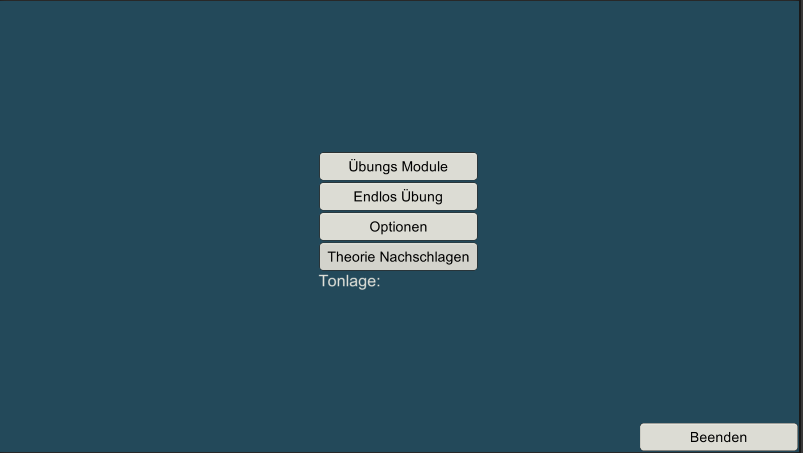
\includegraphics[width=1\textwidth]{Bilder/hauptmenue.png}
    \caption{User Interface des Hauptmenüs}
    \label{sec:hps_algo}
\end{figure}
Wie man erkennen kann ist das Hauptmenü sehr einfach gehalten und bietet lediglich fünf verschiedene Button zur Auswahl an, welche jeweils mit ihrem Ziel beschriftet sind. Es wird außerdem als Schriftzug die gewählte Tonlage des Nutzers angezeigt. Die Buttons rufen jeweils eine Methode des SceneMasters des Hauptmenüs auf, welcher dann die Szene wechselt bzw. die Anwendung beendet. Der SceneMaster setzt ebenfalls den Text der Tonlage. 

\newpage

\subsection*{Einstellungen}
Die globalen Einstellungen dienen vor allem der Konfigurierung der Tonerkennung und der Eingabeparameter, sowie der Tonlage. 
\begin{figure}[H]
    \centering
    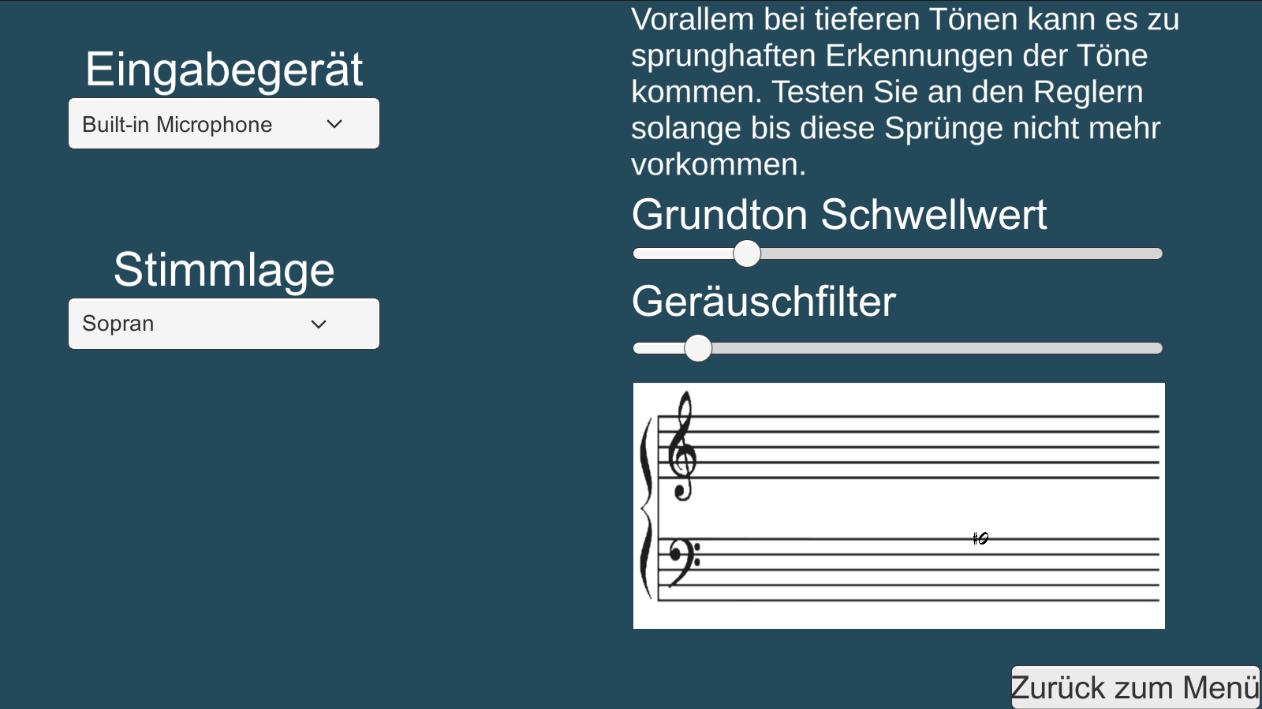
\includegraphics[width=1\textwidth]{Bilder/optionen.png}
    \caption{User Interface der Einstellungen}
    \label{sec:hps_algo}
\end{figure}
Auch diese Szene ist relativ simpel gehalten, mit wenigen UI Elementen und kurzen Erklärungen zu den Reglern. Es wurden zwei Dropdown Menüs eingebunden, welche das Eingabegerät und die Tonlage anpassen können. Weiterhin wurden zwei Slider zum anpassen der Parameter der Tonerkennung hinzugefügt. Der obere Slider, welcher den Schwellwert der Tonerkennung anpasst, kann Zahlen zwischen 0.0001 und 0.5 darstellen, wohingegen der untere Slider eine Reichweite von 0.01 und 0.4 erlaubt. Die Zahlenwerte wurden begrenzt, da bei beiden Slidern ein Wert von 0 oder ein zu großer Wert dazu führt, dass die Tonerkennung nicht mehr funktionsfähig ist. Die genauen Parameter, welche durch diese Slider angepasst werden, werden in einem späteren Abschnitt (\ref{sec:tonerkennung}) genauer erklärt. Es wurde außerdem ein Notensystem in den Optionen platziert, um noch in den Optionen direkt die gewählten Werte überprüfen zu können. Zuletzt wurde auch hier ein Button platziert, welcher zurück auf das Hauptmenü verweist. 

\newpage

\subsection*{Theoriebuch}
Das Theoriebuch soll dem Nutzer als Nachschlagewerk dienen, falls dieser sich zusätzlich zu den Übungen noch zu der Theorie informieren möchte. 
\begin{figure}[H]
    \centering
    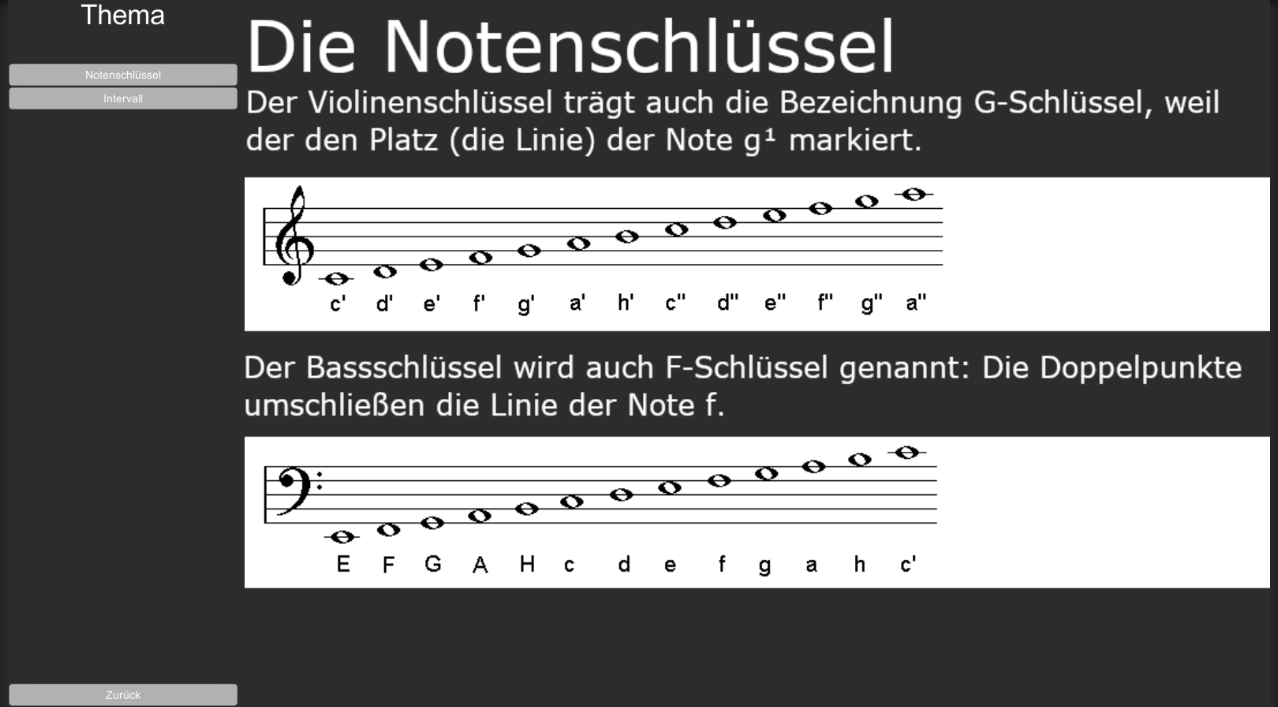
\includegraphics[width=1\textwidth]{Bilder/theorie.png}
    \caption{User Interface des Theoriebuchs}
    \label{sec:hps_algo}
\end{figure}
Das Theoriebuch besteht aus einer Liste an Buttons, welche am linken Bildschirmrand platziert sind. Wird ein Button gedrückt, so wird die Erklärung auf dem Großteil des Bildschirms zu diesem Thema angepasst. Die Erklärungstexte sind prototypisch nur als Grafik eingebunden. Der Button am unteren linken Bildschirmrand führt den Nutzer zurück in die letzte Szene. 

\newpage

\subsection*{Endlosübung und Modulübung}
Die Übungen bestehen im Kern aus dem Notensystem, welches als Eingabe und Ausgabe dient, sowie aus einem kleinen Optionsmenü. Die Endlosübung generiert solange Aufgaben, bis der Nutzer nicht mehr üben möchte, wohingegen die Modulübung ein vordefiniertes Set an Aufgaben stellt. Die UIs der Übungen sind im wesentlichen identisch. 
\begin{figure}[H]
    \centering
    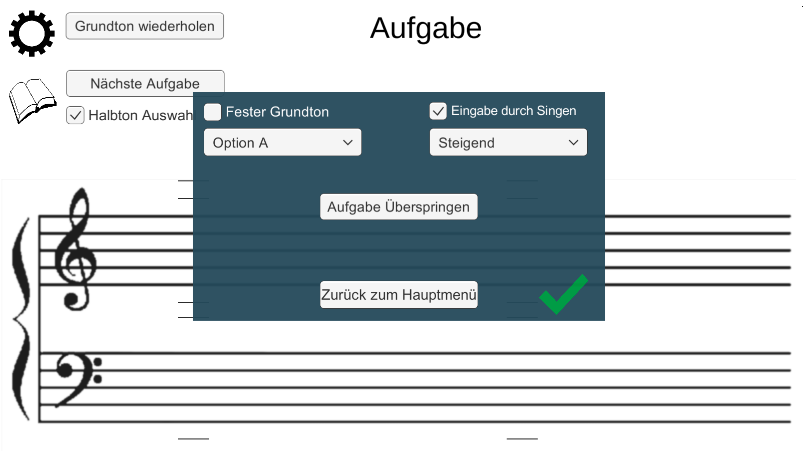
\includegraphics[width=1\textwidth]{Bilder/endlosspiel.png}
    \caption{User Interface der Endlosübung}
    \label{sec:hps_algo}
\end{figure}
Die Übung bietet zunächst über zwei Button an, das lokale Optionsmenü und das Theoriebuch zu öffnen. Betrachtet man das Optionsmenü, so sieht man Buttons, welche die Übung verlassen und das Optionsmenü schließen. Es wird auch die Möglichkeit gegeben, eine Aufgabe zu überspringen, sollte man bei einer Übung nicht weiterkommen. Weiterhin gibt es zwei Dropdownmenüs, welche es zum einen erlauben, den festen Grundton zu definieren und zum anderen die Richtung der Intervalle zu bestimmen. Die zwei Checkboxen lassen sich setzen, um die Eingabemethode zu verändern und das zufällige Wählen der Grundtöne zu stoppen. Alle Komponenten des lokalen Menüs kommunizieren mit dem SceneMaster der Szene, in dem Fall der Übung also dem UIHandler. Dort werden jeweils Methoden aufgerufen, welche den gewählten Wert der Klasse übergeben, von wo diese Werte dann von der Spiellogik abgerufen werden können. \\
Betrachtet man nun die restlichen Teile des UIs der Szene ohne das Optionsmenü, so kann man zwei Buttons sehen, welche das erneute Abspielen des Grundtons ermöglichen und nach dem erfolgreichen Abschließen einer Aufgabe die nächste Aufgabe starten. Der Button, um den Grundton erneut abzuspielen, kommuniziert dabei als einziger nicht mit einem Skript, sondern greift direkt auf die AudioSource in der Szene zu und startet den AudioClip erneut. Die Checkbox zur Eingabe eines Halbtons, welche unter den beiden Buttons liegt, wird nur angezeigt, wenn der Nutzer mit der Maus eine Note setzen möchte und dadurch auch Halbtöne setzen können muss. Weiterhin lässt sich ein Textfeld am oberen Rand der Szene erkennen, in welchem später die Aufgabenstellungen angezeigt werden. Ebenso liegt rechts neben diesem Textfeld ein weiteres Textfeld, in welchem der Nutzer Informationen bzw. Feedback erhält. Ist die Aufgabe richtig beantwortet, so wird dort beispielsweise kommuniziert, dass sie bestanden wurde. Auf das Notensystem werde ich in Kapitel \ref{sec:notensys} genauer eingehen. 

\section{Implementierung der Systemkomponenten}
Im Folgendenen wird die Entwicklung der prototypischen Trainingssoftware zur Gehörbildung näher beleuchtet und der Prozess der Umsetzung der Konzeption gezeigt. Ich werde die konzipierten Systemkomponenten ansprechen und darauf eingehen, wie diese umgesetzt wurden. 
In Unity gibt es die sogenannte MonoBehaviour Superklasse, welche einige Funktionen implementiert welche die Unityengine zu bestimmten Zeiten aufruft, wenn ein Skript, welches von MonoBehaviour erbt, in einer Szene eingebunden ist. Zu den wichtigsten Funktionen zählen die Funktion Start() und Update(). Start wird automatisch einmal während der Initialisierung des Skripts aufgerufen, wohingegen Update in jedem Frame genau einmal aufgerufen wird. Es existieren noch weitere Funktionen, wie etwa die Funktion FixedUpdate(), welche unabhängig von der Framerate in einem fixen Zeitintervall aufgerufen wird.

\subsection*{Notensystem}
\label{sec:notensys}
Das Herzstück der Ein- und Ausgabe bildet das Notensystem. Da dieses nicht nur als Anzeige des Grundtons verwendet werden sollte, sondern zusätzlich entweder als Anzeige des gesungenen Tons oder als Eingabe des Tons mit der Maus. Umgesetzt wurde dieses komplexe Modul im wesentlichen in zwei Klassen. Diese sind zum einen die Klasse OnehotNote und zum anderen der NoteSystemHandler. Wie der Name der OnehotNote bereits erahnen lässt, implementiert diese das oben beschriebene Verhalten für eine einzelne Note, wobei immer nur eine Note aktiv sein darf. Wie man in der Abbildung erkennen kann, hat jede der Noten eine \glqq Hitbox'' in welcher sie auf dem Notensystem liegt. Diese Hitbox wird mithilfe eines Box Colliders umgesetzt, welcher es innerhalb der OnehotNote Klasse erlaubt abzufragen, ob die Maus über dem Boxcollider hovert. In der folgenden Abbildung kann man die Boxcollider sehr gut an den grünen Boxen innerhalb des Notensystems erkennen. Weiterhin kann man die Struktur des Notensystem Gameobjects sehen. Es wurden zwei Blöcke an Hitboxen zur Erkennung der Noten implementiert, wobei alle Notenobjekte den gleichen Skriptcode verwenden können, da der NotesystemHandler die jeweiligen OnehotNotes so initialisiert, dass diese das richtige Verhalten aufweisen. Jede Note hat Zugriff auf den assoziierten SpriteRenderer, um den Notenkopf bei verändertem Vorzeichen anzupassen, welcher vom NotesystemHandler gesetzt bzw. bezogen werden kann. Weiterhin hat die Note Zugriff auf den Boxcollider, um die Methoden OnMouseEnter, OnMouseExit, sowie OnMouseDown implementieren zu können. Um sicherzustellen, dass immer nur die Note ihren Sprite setzt, welche gerade tatsächlich gewollt ist, werden die booleschen Parameter StayOn, StayOff und EnableClickIn gesetzt. 

\begin{figure}[H]
    \centering
    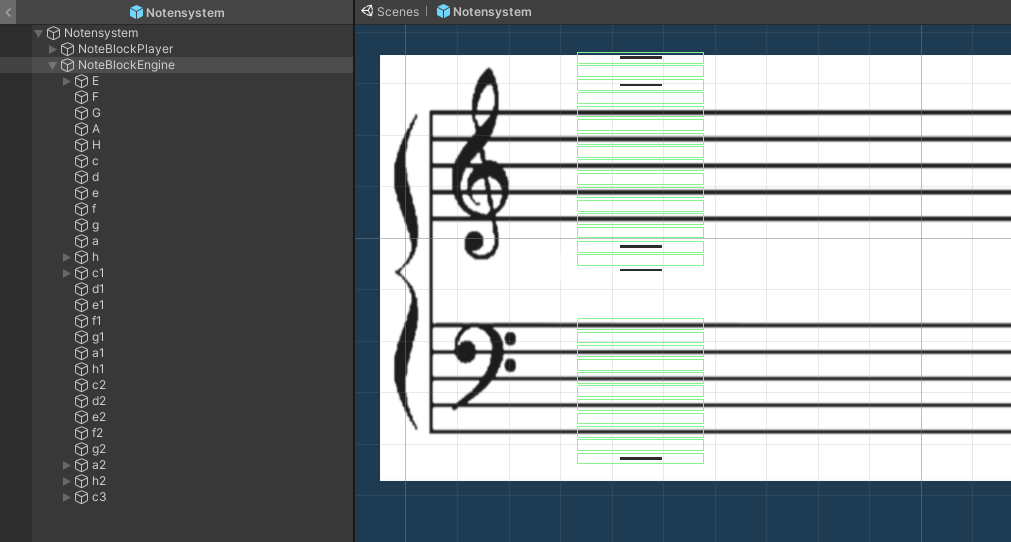
\includegraphics[width=1\textwidth]{Bilder/notensystem.png}
    \caption{Aufbau des Notensystems in Unity}
    \label{sec:hps_algo}
\end{figure}

Während der Initialisierung des Notensystems setzt dieses bei allen Noten zunächst den Parameter EnableClickIn. Dieser sorgt dafür, dass der linke Notenblock nicht auf die Maus reagiert, der rechte Notenblock jedoch schon. Klickt der Nutzer auf eine Note, so wird dabei der Parameter StayOn dieser negiert, sodass eine nicht angewählte Note angewählt bleibt oder eine angewählte Note wieder freigegeben wird und nicht mehr angezeigt wird. Bei dieser Aktion wird gleichzeitig dem Notensystem der gleiche Wert übergeben, woraufhin der NotensystemHandler bei allen anderen OnehotNotes den Parameter StayOff setzt. Will man bei einer Note den Wert im Notensystem durch klicken setzen, müssen alle drei dieser Parameter negativ sein, damit die Note gesetzt werden kann. \\
Ist die Option zum Singen aktiviert, so kann der NotesystemHandler auch alleine extern alle Noten so ansteuern, dass der gesungene Ton angezeigt wird. Möglich gemacht wird dies durch die öffentlichen Methoden RenderNote, AddFlat, AddSharp, sowie ResetSprite. Über diese Methoden ist es möglich, jegliche Veränderungen an dem Sprite durchzuführen und die Note somit extern zu setzen. Das Notensystem erfüllt somit sowohl die Aufgabe der Eingabe, als auch die Ausgabe. Der NotesystemHandler bezieht jedoch nicht selbst die Mikrofondaten, sondern stellt lediglich der Gamelogic eine Methode zur Verfügung um den gewünschten Ton setzen zu können. Der Ton muss in dem normierten internen Format als Integer übergeben werden. Er wird dann zunächst daraufhin überprüft, ob er einen Halbton darstellt. Ist das der Fall, wird bei der Wahl des Notenobjekts darauf geachtet, ob die Aufgabe Intervall nach oben oder unten vervollständigt erwartet, um dann schließlich die richtige Note mit dem passendem Vorzeichen auszuwählen. Es wird außerdem die zuletzt vom Spieler gesungene Note gespeichert, um einige Rechenschritte zu sparen, sollte Sie mehrmals hintereinander gesetzt werden. 


\subsection*{Schnittstellen}
Es wurden zwei Schnittstellen implementiert, welche jeweils Inputdaten und Outputdaten sammeln und setzen. Der InputHandler hat Zugriff auf den FrequencyHandler, das Notensystem und den UIHandler, um von diesen alle relevanten Daten beziehen zu können. Es wird in jedem Frame die gesungene Frequenz, die erkannte Note, die mit der Maus ausgewählten Note, sowie die Optionen des UI gespeichert. Diese Werte werden anderen Klassen öffentlich zum Lesen zur Verfügung gestellt. \\
Die Outputschnittstelle übernimmt während des Spiels die Aufgabe, die Daten richtig in der Szene zu platzieren. Die Spiellogik muss dafür nur die notwendigen Daten dem UIHandler übergeben. Um eine Aufgabe vollständig anzuzeigen, sind lediglich der geforderte Ton, der dazugehörige Grundton und das Intervall zwischen diesen Tönen zu übergeben. Der UIHandler setzt anschließend auf dem Notensystem den Grundton, sowie den gesungenen Spielerton und passt den Text der Aufgabe an, sodass das geforderte Intervall abgefragt wird. Es ist außerdem möglich, von der Spiellogik einen angepassten Aufgabentext zu übergeben, welcher für das modulbasierte Lernen notwendig ist. Bei dem modulbasierten Modus liest die Spiellogik einen anpassbaren Aufgabentext aus einer .json. Dieser Text kann dann über diese alternative Methode gesetzt werden. 

\subsection*{Generierung der Töne}
Die Generierung der Töne erfolgt komplett isoliert innerhalb einer Klasse, welche lediglich eine Methode zur Verfügung stellt. Die Spiellogik kann die Methode PlayFreq mit einer Frequenz aufrufen, woraufhin ein Sinuston mit einer Samplerate von 44100 Hz berechnet wird. Um einen Sinuston zu berechnen, muss lediglich über die gesamte Länge der Samples eine Sinuswelle gelegt werden. Es wird dementsprechend ein Array mit 44100 Felder, gefüllt
$$\text{ton}[i] = \sin(\frac{2 * \pi * i * F}{F_s})$$ 
wobei $i$ der Index des Arrays, $F$ die Frequenz des zu berechnenden Tons und $F_s$ die Samplerate, also 44100, ist.\\
Dieser Ton wird nach der Berechnung direkt einer AudioSource als Clip hinzugefügt und die AudioSource im Anschluss ausgeführt. Diese Umsetzung ermöglicht das mehrfache Abspielen des Tons, mit einer einmaligen Berechnung, da der Ton immer in der AudioSource gespeichert wird. 

\subsection*{GUI Masterskripte}
Die sogenannten SceneMaster existieren in jeder Szene genau einmal und übernehmen allgemeine Aufgaben des UI und der Szenenkontrolle, wie etwa ein Szenenwechsel, sowie die Kommunikation mit dem SceneHandler, welcher globale Daten speichert. Im Fall der Spielszenen sind die SceneMaster die bereits angesprochenen UIHandler. Im Fall des SceneMasters des Hauptmenüs, implementiert dieser vor allem Methoden, welche das Wechseln von Szenen erlauben, sodass diese von einem Button aufgerufen werden können. Es wird zum Wechseln einer Szene lediglich der Aufruf der statischen Klasse SceneHandler mit dem Szenennamen als Übergabeparameter benötigt. Außerdem setzt er einige globale Werte, welche notwendig sind um das Spiel zu starten. Im Fall des Theoriebuchs werden öffentliche Methoden implementiert, welche das Wechseln zwischen den einzelnen \glqq Buchseiten'' ermöglicht. Der SceneMaster der Optionenszene setzt ebenfalls vor allem Methoden um, welche das setzen von globalen Werten ermöglichen, wie etwa die angepassten Parameter der Tonerkennung.  

\subsection*{Gamelogic}
Da es zwei verschiedene Spielmodi gibt, mussten auch zwei unterschiedliche Gamelogicklassen geschrieben werden, welche jedoch viele Gemeinsamkeit teilen und daher von einer Elternklasse erben können. Die Elternklasse \glqq BaseGameLogic'' implementiert die notwendigen Schnittstellen zu anderen Klassen, sowie die äußerst wichtige Methode \glqq RefreshInputVals''. Gamelogic hat Zugriff auf die Utility Klassen und auf die Datenstrukturen, sowie auf den Tongenerator und den Inputhandler. Außerdem kann die Gamelogic Klasse auf einen JsonLoader zugreifen und auf den UIHandler. Die Methode \glqq RefreshInputVals'' ist wichtig, da diese nach jeder UI - Eingabe die Gamestate relevanten Parameter neu setzt, um so die vom Nutzer eingegebenen Werte aus dem UI spätestens im nächsten Frame schon zu übernehmen. Es kann bei den Parametern zu einer Veränderung des Grundtons der Aufgabe kommen, falls der Nutzer diesen selbst wählen möchte, statt ihn zufällig generieren zu lassen. Tritt dieser Fall ein, so muss eine neue Aufgabe generiert werden, welche den fest gewählten Grundton verwendet. Die Methode überprüft daher bei jedem Aufruf, welcher Grundton verwendet werden muss und passt diesen dementsprechend an. Es werden die zwei virtuellen Methoden \glqq NextExer'' und \glqq NextExerButton'' vorgegeben, welche in den Unterklassen zu definieren sind. Es handelt sich bei diesen Methoden um die Anbindung zum Button, um die nächste Übung zu beginnen (NextExerButton) und der Methode, welche alle Parameter setzt und Funktionsaufrufe tätigt, um die nächste Übung zu generieren und anzuzeigen (NextExer). Es werden auch nicht-virtuelle Methoden implementiert, die bestimmte Sachverhalte umsetzen, die für alle Spielmodi gleich sind. Unter diese fallen neben RefreshInputVals auch Methoden zum Beziehen des Inputs aus der richtigen Quelle und zur Überprüfung der Aufgabe. Es wird außerdem eine zeitlich abhängige Überprüfung der Aufgaben implementiert, welche das richtig Beantworten der Aufgabe nur zulässt, wenn der Nutzer die richtige Note lang genug gesungen hat. Diese Überprüfung wird mithilfe der Unity internen Zeit umgesetzt, indem eine Flag gesetzt wird, wenn das erste Mal der Ton gesungen wird und in den folgenden Frames überprüft wird, ob die Zeit zwischen der ersten Eingabe und der neuesten Eingabe bereits die Zeit der Aufgabe erreicht. Ist das der Fall, wird die Flag gesetzt, dass die Aufgabe gelöst wurde. Die Unterklassen der verschiedenen Spielmodi müssen lediglich die zwei vorgestellten virtuellen Methoden überschreiben.\\
Die Spiellogik für das Endlosspiel ruft in jedem Frame die Methode zur Überprüfung der gehaltenen Noten in der Elternklasse mit dem Input auf. Wenn die Aufgabe gelöst ist, wird dem Nutzer Feedback über eine Ausgabe gegeben und dazu aufgefordert, den Button zur nächsten Aufgabe zu drücken. Der Button führt dann die erste der überschriebenen Methoden aus (NextExerButton), welche überprüft, ob die Aufgabe tatsächlich abgeschlossen wurde ist das der Fall wird NextExer aufgerufen. NextExer generiert eine neue Aufgabe, basierend auf den Präferenzen des Nutzers, und startet die nächste Aufgabe mit dem Abspielen des Grundtons. \\
Ähnlich wie das Endlosspiel ruft auch die Spiellogik der Module in jedem Frame die Überprüfung der gehaltenen Noten mit dem Input auf. Der Ablauf der Überprüfung ist identisch bis zu dem Punkt, an dem der Nutzer auf den Button zur nächsten Aufgabe klickt, woraufhin auch hier die Methode NextExerButton aufgerufen wird. Der Unterschied dieser Implementierung der Methode im vergleich zu der des Endlosspiels liegt in der weiteren Überprüfung, ob diese Aufgabe abgeschlossen wurde oder nicht. Es wird hier zusätzlich überprüft, ob das letzte Modul vollendet wurde. Wurde das letzte Modul beantwortet, ruft die Methode den SceneHandler auf, um die Szene zum Hauptmenü zu wechseln. Ist das jedoch nicht der Fall, so wird auch hier die Methode NextExer aufgerufen um die nächste Aufgabe zu setzen. Der Unterschied der Methode NextExer zu ihrem Pendant liegt darin, dass hier die Bestandteile der Aufgabe aus der eingelesenen .json Datei gesetzt werden müssen. 

\subsection*{Datenstruktur und Hilfsklassen}
Ich fasse in dieser Sektion einige Klassen zusammen, welche keinen direkten Einfluss auf das Spiel nehmen, sondern als Hilfsklassen bestimmte Daten oder Methoden zur Verfügung stellen. Sie haben somit keinen Zugriff auf andere Klassen. Eine der wichtigsten dieser Klassen ist der bereits angesprochene SceneHandler. Der SceneHandler ist eine statische Klasse, welche dadurch globale Parameter für alle Szenen speichert und den Austausch dieser untereinander ermöglicht. Der SceneHandler speichert das gewählte Mikrofon, die Tonhöhe des Nutzers, die Einstellungen der Tonerkennung und die zuletzt aufgerufene Szene. Es werden demnach nur Parameter aus der \glqq Optionen'' - Szene gespeichert. Weiterhin implementiert der SceneHandler Methoden zur Szenennavigation, welche das gezielte wechseln in eine andere Szene und das Wechseln in die letzte Szene ermöglichen. Ein Szenenwechseln in Unity geschieht über die interne Klasse SceneManager mit dem Methodenaufruf LoadScene. \\
Es werden außerdem Klassen zum Berechnen einer einfachen Newton Interpolation und zum Initialisieren des .json File Readers implementiert. Im  gFall der Interpolation handelt es sich um eine herkömmliche Implementierung \cite{newtonInterpolation}. Der JsonLoader stellt lediglich eine Methode zur Verfügung, welche die eingelesenen Daten der .json Datei in dem Format der Datenstruktur zurückgibt. \\
Eine weitere wichtige Hilfsklasse ist die FrequencyUtil Klasse. Die Klasse stellt allen Klassen, welche mit Frequenzen arbeiten müssen, diverse Methoden zur Berechnung einzelner Werte zur Verfügung. Es werden Methoden zur Intervallberechnung zur Verfügung gestellt, sowie Methoden, welche zufällige Töne oder Intervalle zurückgeben. Eine der wichitgsten Methoden ist die GetNearestNoteFromFreq Methode diese rundet eine Frequenz zu dem nächsten definierten Ton. Die Methode wird immer dann benötigt, wenn ein nicht bereinigter gesungener Ton vom Nutzer eingelesen wird, da man von dem Nutzer nicht eine 100 prozentige Genauigkeit erwarten kann. Die Methode iteriert dabei durch ein Array, welches alle Frequenzen der gleichstufigen Stimmung beinhält und findet den geringsten Abstand zu der übergebenen Note. Da die Frequenzen als Integer in der Datenstruktur abgespeichert werden mussten, wurde diese normalisiert, indem sie mit dem Faktor 100 multipliziert wurde. FrequencyUtil stellt daher Methoden zur Verfügung, um zwischen dem normalisierten Format und der echten Frequenz zu unterscheiden. \\
Abschließend sind noch die Definitionen der Datenstrukturen zu erwähnen. Es werden innerhalb der Datastructures Klasse die Definitionen der gleichstufigen Intervalle und der korrespondierenden Frequenzen als enum gespeichert. Aufgrund der großen Anzahl an Verwendungen dieser Daten wurde entschieden, diese permanent als enum einzupflegen. Weiterhin werden auf der Basis der gespeicherten Frequenzen anschließend die Tonlagen mithilfe dieser modelliert und zusätzlich einige Hilfsmethoden zu den Tonlagen geschrieben. Die Hilfsmethoden sind vor allem zur Darstellung der Tonlagen als String Array bzw. als Array, welches die Objekte der Tonlagen speichert. Außerdem wurde eine Methode entwickelt, welche alle Frequenzspektrum innerhalb der Tonlage zurückgibt. Es wurde zusätzlich das Format der .json Datei definiert, sodass diese erfolgreich eingelesen werden kann. 

\section{Tonerkennung}
\label{sec:tonerkennung}
Die Tonerkennung wurde mithilfe von zwei Klassen umgesetzt, welche von der Klasse MonoBehaviour erben und jeweils ein eigenes GameObject in der Spielszene darstellen, sowie einer AudioSource, welche ebenfalls als alleinstehendes GameObject in der Szene existiert. Wie bereits in der Konzeption beschrieben, hat die Klasse FrequencyReader die Aufgabe, das Mikrofon zu initialisieren, wohingegen die Klasse FrequencyHandler die tatsächliche Tonerkennung durchführt. \\
FrequencyReader implementiert ein öffentliches Attribut \glqq playback'', welches die AudioSource mit den geladenen Mikrofondaten repräsentiert und eine Konstante \glqq SampleRate'', welche die Samplerate von 44100Hz festlegt und freigibt. Die Klasse implementiert nur die Funktion Start(). Es werden in Start() das gewählte Eingabegerät aus dem SceneHandler abgerufen und daraufhin der AudioClip von playback direkt gesetzt. Es muss dann noch der Parameter loop der AudioSource playback auf true gesetzt werden. Dieser Parameter ermöglicht es, dass die AudioSource den festgelegten Clip unendlich oft wiederholt und nicht nach einem Durchlauf abbricht. Es muss abschließend noch die Position der Daten des Mikrofons solange gepollt werden, bis Daten vorliegen und die AudioSource abgespielt werden. Der aufgenommene Clip muss über eine AudioSource abgespielt werden, sodass die AudioDaten aus dem Mikrofon übernommen werden können. Ab diesem Punkt führt die Klasse FrequencyHandler den bereits vorgestellten Algorithmus (\ref{pda}) auf den AudioDaten des Mikrofons aus. Es wird die berechnete Frequenz, sowie die korrespondierende Note anderen Klassen zur Verfügung gestellt. 

\begin{algorithm}[H]
    \caption{Pitch Detection Algorithm} \label{pda}
   \begin{algorithmic}[1]
    \Require {filter, threshold, cutoff}
    \Function {ComputeFrequency}{}
        \State spectrum=GetSpectrumData()
        \State spectrumCut = first values of spectrum till cutoff Value 
        \State absMaxIndex = 0 
        \State max = maximum of spectrumCut
        \State avg = average of spectrumCut
        \For{$i = 1$ \textbf{to} length of spectrumCut $- 1$} 
            \If{spectrumCut[i] < avg $*$ filter} 
                \State spectrum[i] = 0
                \State \textbf{continue} to next iteration
            \EndIf
            \If{spectrumCut = max}
                \State absMaxIndex = i
            \EndIf
        \EndFor
        \State bestIndex = HandleOvertones(absMaxIndex)
        \State interpolatedIndex = Interpolate(bestIndex)
        \If{interpolatedIndex != 0}
            \State \textbf{return} interpolatedIndex $* \ F_c$
        \EndIf
        \State \textbf{return} bestIndex $* \ F_c$
   \EndFunction
    \State
    \Function{HandleOvertones}{absMaxIndex}
        %\Require absMaxIndex, spectrum\_cut
        \State overtoneMax = 0
        \State overtoneMaxIndex = absMaxIndex
        \For{i = absMaxIndex \textbf{to} 1}
            \State currentVal = spectrumCut
            \If{currentVal = 0}
                \State overtoneMax = 0
            \EndIf
            \If{currentVal > spectrumCut $*$ threshold}
                \If{overtoneMax < currentVal}
                    \State overtoneMax = currentVal
                    \State overtoneMaxIndex = i
                \EndIf
            \EndIf
        \EndFor
        \State \textbf{return} overtoneMaxIndex
    \EndFunction
\end{algorithmic}
\end{algorithm}
\newpage
\subsection*{Berechnung der Laufzeitkomplexität des vorgestellten Algorithmus}
Es gilt zu zeigen, dass der vorgestellte Pitch Detection Algorithmus effizient ist. Ich werde die Funktion \glqq HandleOvertones'' zunächst untersuchen, da diese von der Funktion \glqq ComputeFrequency'' aufgerufen wird. Man kann sehen, dass die Zeilen 25 und 26, sowie die Zeile 39 nur einmal pro Ablauf aufgerufen werden und daher vernachlässigbar sind. Sei n die Länge des Spektrums. Die Schleife wird im worst case Szenario $n$ mal und die Zeile 27 $n + 1$ durchlaufen. 
$$3 * \mathcal{O}(1) + 7 * \mathcal{O}(1) * \mathcal{O}(n) + \mathcal{O}(1) = \mathcal{O}(n) $$
Die Laufzeitkomplexität der Funktion beläuft sich demnach auf $\mathcal{O}(n)$. Die Komplexität der Funktion \glqq ComputeFrequency'' werde ich zunächst betrachten, ohne auf die Funktionsaufrufe einzugehen. Die Schleife in dieser Funktion wird immer $n$ mal und die Zeile 7 $n + 1$ ausgeführt. Alle anderen Zeilen werden nur einmal ausgeführt, sodass auch hier eine Schranke von $\mathcal{O}(n)$ gesetzt werden kann. Die aufgerufenen Funktionen sind jedoch nicht so laufzeiteffizient. Berücksichtigt man noch die Funktionsaufrufe, so stellt man schnell fest, dass die Laufzeitkomplexität höher ausfällt. Geht man davon aus, dass GetSpectrumData eine gewöhnliche rekursive FFT berechnet, so beläuft sich die Laufzeitkomplexität dieser auf $\mathcal{O}(n \log{n})$. Eine Newton Interpolation hat sogar eine maximale Laufzeitkomplexität von $\mathcal{O}(n^2)$; diese Laufzeitkomplexität begründet auch, warum nur drei Punkte interpoliert werden. Da die Anzahl der zu interpolierenden Punkte fest ist, werde ich die Laufzeitkomplexität der Interpolation als konstant annehmen. Die Komplexität der Max, Avg und Copy Funktionen sind ebenfalls linear.
$$\mathcal{O}(n \log{n}) + 4 * \mathcal{O}(n) + 5 * \mathcal{O}(1) + 5 * \mathcal{O}(1) * \mathcal{O}(n) = \mathcal{O}(n \log{n})$$
Den größten Einfluss auf die Zeitkomplexität nimmt die von Unity zur Verfügung gestellte Funktion, sodass der Algorithmus nicht weiter optimiert werden kann, da diese Funktion essenziell ist.



\chapter{Validierung der erarbeiteten Methoden und Konzepte}

%- Mehrstufige Validierung mit Musikverein, Studenten, ...
%- Unterschiedliche Validierungen vergleichen
%- Konzept in 3 Stufen
%-- Vorbereitung, Durchführung, Nachbereitung
%-> Wie gemacht: Was will ich messen(ERkennungsrate, UX Bewertung)
% Auf quintessenz eingehen, gesamte Eval. in den Anhang
% nenne samplegröße, durchschnittsalter, frau/mann zusammensetzung
Im folgenden Kapitel werde ich zunächst auf die unternommenen Maßnahmen zur Vorbereitung der Evaluation eingehen. Im nächsten Schritt wird die Durchführung der Evaluation näher erläutert und die Entscheidungsfindung der Durchführungsart beleuchtet. Schließlich werden die Ergebnisse der Evaluation ausgewertet und hinsichtlich der zu untersuchenden Punkte gedeutet.  Das Ziel der Evaluation soll sein, die implementierte Tonerkennung in Unity auf eine möglichst großen Menge an Systemen testen zu können und somit die Echtzeitkomponente der Anforderung überprüfen zu können. 
\section{Evaluationskonzept}
%    - Hobby, Profi, Studierende
%    - Unterschiedliche Fragen für jede Gruppe? oder Unterschiedliche Wahrnehmung der Gruppen?
%    - Hobby
%        - Dazu gelernt? Hilfreich? Richtige Kompetenz oder zu schwer?
%    - Profi
%        - Soetwas gewünscht in der Ausbildung? Weiterhin praktisch zum fit bleiben? Empfehlung an Kollegen?
%    - Studierende  
%        - Richtige Ansätze für Uni? Hilfreich beim Lernen? Alle wichtigen Features dabei?
%    -allgemeine
%        - Wie war die Erkennung der Stimme
%        - Nutzbarkeit der Anwendungen
%       - Weiter verwenden?
Ziel der Evaluation soll sein, die erarbeitete Tonerkennung auf ihre Genauigkeit hin mit möglichst verschiedenen Stimmlagen zu überprüfen. Um eine möglichst breite Evaluationsgruppe sicher zu stellen, möchte ich vor allem drei Gruppen an Musikern die Evaluation durchführen lassen. Diese drei Gruppen sind Hobbymusiker, professionelle Musiker und Musikstudenten. Dabei habe ich an jede Gruppe andere Ansprüche und möchte auf die individuellen Bedürfnisse und Umstände dieser in der Evaluation eingehen. Daraus erhoffe ich mir ein möglichst breites Bild zu der Umsetzung der Trainingssoftware zu machen und somit auch ein aussagekräftiges Fazit ziehen zu können.
Ich habe die genannten Gruppen ausgewählt, da diese einen großen Teil der praktizierenden Musiker abdecken, aber auch unterschiedliche Instrumente und Musikarten abdecken können. Gerade die Studierenden sind in Bezug auf die Trainingswirkung interessant, da diese häufig im Studium das Modul Gehörbildung absolvieren müssen und sie daher einen näheren Bezug zu anderen Lernmethoden haben. \\
\subsection{Hobbymusiker}
Ich möchte bei Hobbymusikern vor allem auf ihre vorhandene Motivation und neu erlangte Motivation durch das Trainingsprogramm eingehen. Außerdem möchte ich herausfinden, ob die vorausgesetzten Kompetenzen zu hoch waren und ob diese durch das Programm dennoch gefördert werden konnten. Ich gehe bei Hobbymusikern dabei am ehesten davon aus, dass sich diese noch nie oder nur im Instrumentalunterricht, mit Gehörbildung beschäftigt haben. Auf dieser Grundlage ist es für mich interessant, ob das entwickelte Trainingsprogramm sie dazu anregen konnte, sich etwas näher mit Gehörbildung auseinanderzusetzen und ob sie denken, dass sie in der Ausübung ihres Hobbys einen Mehrwerte daraus ziehen können. Mithilfe dieser Fragestellungen versuche ich darauf zu schließen, ob die Motivation, sich mit Gehörbildung auseinanderzusetzen gesteigert werden konnte. In dem Zusammenhang ist es auch wichtig, wie stark die Aufgaben die Anwender gefordert haben.
\subsubsection*{Kernfragen}
\begin{itemize}
    \item Wie ist die Motivation zur Gehörbildung vor und während der Anwendung der Trainingssoftware gewesen?
    \item Waren die vorausgesetzten Kompetenzen zu hoch? Falls ja, konnten diese dennoch durch das Programm gefördert werden?
    \item Konnte das Programm die Motivation steigern, sich mehr mit Gehörbildung auseinanderzusetzen?
    \item Lässt sich aus dem Training ein Mehrwert für das eigene Hobby ziehen?
\end{itemize}
 
\subsection{Studierende}
Die Meinung der Studierenden ist mir vor allem in Bezug auf das Musikstudium und spezifisch auf Gehörbildung wichtig. Ich erhoffe mir, von Studierenden den Nutzen für das Studium zu erfahren und was sie sich an einer solchen Anwendung noch zusätzlich wünschen würden. Außerdem möchte ich von Studierenden erfahren, ob die Anwendung das Wissen abfragt, welches von ihnen verlangt wird und sie dementsprechend lernen müssen. Es ist bei Studierenden wichtig, dass das benötigte Wissen gut und schnell vermittelt bzw. trainiert wird. Ich möchte an diesen Fragestellungen daher vor allem die tatsächliche Trainingswirkung im Vergleich zu den aktuell angewandten Methoden messen können.
\subsubsection*{Kernfragen}
\begin{itemize}
    \item Wie hoch ist der Nutzen für das Musikstudium?
    \item Was sind zusätzliche Wünsche bezüglich des Studiums, die an der Anwendung fehlen?
    \item Wird das gleiche Wissen abgefragt wie im Studium?
\end{itemize}

\subsection{Professionelle Musiker}
Als letzte Gruppe möchte ich versuchen, einige professionelle Musiker zu befragen. Ihre Meinung ist besonders dahingehend interessant, ob sie sich vorstellen können, dass ihnen eine solche Software in dieser Zeit geholfen hätte. Außerdem möchte ich wissen, ob sie sich vorstellen können so Gehörbildung weiterhin zu trainieren. Diese Fragen verfolgen ein ähnliches Ziel, wie die der Studierende, jedoch zählt in die Antworten der professionellen Musiker noch die Erfahrung mit hinein.   
\subsubsection*{Kernfragen}
\begin{itemize}
    \item Hätte eine solche Anwendung während der Ausbildung zum professionellen Musiker geholfen? 
    \item Ist diese Art des Trainings der Gehörbildung förderlich für einen professionellen Musiker?
    \item Benötigen professionelle Musiker auch nach der Ausbildung so eine Anwendung?
\end{itemize}

\subsection{Allgemeine Fragen}
Abschließend gibt es einige Aspekte zu erwähnen, welche alle der oben genannten Gruppen betreffen und sie dementsprechend alle beantworten können. Unter diese Aspekte fallen die allgemeinen Punkte der Software, wie etwa die Performance oder die Zufriedenheit mit der Tonerkennung. Weiterhin fallen unter die allgemeinen Punkte, wie gut die Nutzer mit der generellen Handhabung der Software zurecht kamen und ob sie planen, die Software weiterhin zu verwenden. Weiterhin ist es wichtig grobe Angaben zu der verwendeten Hardware zu erhalten. Falls die Tonerkennung nicht wie gewünscht funktioniert hat lassen sich so hoffentlich Zusammenhänge zu nicht optimaler Hardware herstellen. Die allgemeinen Fragen sollen vor allem abfragen, ob die technischen Ziele und entworfenen User Experience Designs erreicht wurden.
\subsubsection*{Kernfragen}
\begin{itemize}
    \item Wie performant lief die Anwendung?
    \item Als wie genau wurde die Tonerkenung empfunden?
    \item Wie gut kam der Nutzer mit der Handhabung der Anwendung zurecht? War die User Experience angenehm?
    \item Wird geplant die Anwendung weiterhin zu verwenden?
    \item Welches Mikrofon wurde zum Singen verwendet? Wie wurde es mit dem Computer verbunden?
    \item Hat das Spielen Spaß gemacht?
\end{itemize}

\section{Vorbereitung}
Die Evaluation soll über dem Zeitraum von einem Monat durchgeführt werden. Die Durchführung wird jeweils bei den Testpersonen lokal stattfinden und nicht an einem zentralen Ort durchgeführt werden. Die Ergebnisse sollen zur Evaluation des Abschlusses der Programmentwicklung verwendet werden, um somit die angestrebten Maßnahmen zu überprüfen. 
Da die Evaluation nicht fest an einem Standort unter Idealbedingungen durchgeführt wird, sondern bei jedem Nutzer lokal auf den eigenen Geräten, ist es wichtig, die Anwendung zunächst für eine möglichst große Menge an Endnutzergeräten zur Verfügung zu stellen. Die Anwendung wird dementsprechend für die Betriebssysteme Windows 10 (32 Bit), Windows 10 (64 Bit) und für OSX exportiert. Zusätzlich zu der Anwendung erhält jeder Anwender ein Dokument, in welchem beschrieben wird, wie die Anwendung auszuführen ist, sowie eine Bedienungsanleitung zu der Anwendung. Die Bedienungsanleitung geht auf das Einstellen der Tonerkennung, sowie mögliche Lösungsansätze, falls diese die Stimme bzw. den Ton nicht genau erkennen kann ein. Weiterhin werden die zwei Übungsmodi beschrieben und wie diese zu verwenden sind. Außerdem ist in der Anleitung auch der Link zu der online Evaluation vorhanden. Es musste außerdem basierend auf der Konzeption der Evaluation ein Fragebogen erstellt werden, welcher die zu überprüfenden Punkte abfragt. Der Evaluationsbogen wurde mithilfe von Google Forms erstellt, wie auch die folgenden Grafiken der Evaluation. Die Daten werden in drei verschiedenen Arten erhoben. Zum einen in der Form von einer Zufriedenheitsskala, welche zwischen fünf Zufriedenheitszuständen unterscheidet. So kann eine Frage mit einer Zufriedenheit von 1 bis 5 bewertet werden, was mit \glqq Trifft gar nicht zu'' bis \glqq Trifft voll zu'' korrespondiert. Weiterhin werden auch multiple choice Fragen mit einer und mehreren gleichzeitig auswählbaren Antwortmöglichkeiten gestellt. Es werden zudem Textantworten bei einzelnen Fragen erlaubt. 

\section{Durchführung}
Nach dem Starten der Anwendung sollen die Tester zunächst die Optionen aufrufen, sich dort mit der Tonerkennung vertraut machen und diese auf Ihre Stimme einstellen. Weiterhin müssen sie dort die allgemeinen Einstellungen setzen, welche die Tonlage und das Eingabegerät betreffen. Daraufhin werden die Tester aufgefordert, die modulbasierte Übung zunächst zu spielen, wo sie eine Einführung zu Intervallen erhalten. Die fundamentalen Grundlagen sind somit gesetzt, um den Endlosübungsmodus solange zu testen, wie es dem Tester beliebt. Die Tester sollen vor allem die Tonerkennung verwenden, um mit der Anwendung zu interagieren. Zuletzt wird der Tester aufgefordert, den erhaltenen Fragebogen auszufüllen und abzuschicken. 

\newpage
\section{Auswertung}
Bei der Auswertung werde ich auf einige wichtige Fragestellungen eingehen und gegebenenfalls Werte aus anderen nicht aufgelisteten Ergebnissen nur nennen. Der gesamte Evaluationsbogen der zusammengefassten Ergebnisse ist ebenfalls im Anhang einsehbar. \\
An der Evaluation haben 19 Personen teilgenommen, welche zwischen 16 und 59 Jahren alt waren. Unter den Teilnehmern waren 12 männliche und 7 weibliche Personen. Die Teilnehmer waren zusammengesetzt aus 11 Hobbymusikern, 5 Studenten und 3 professionellen Musiker. Bei allen folgenden Grafiken, steht eine Bewertung von 5 für \glqq trifft voll zu'' und eine Bewertung von 1 für \glqq trifft gar nicht zu''.

\subsection*{Hobbymusiker}
\begin{figure}[H]
    \centering
    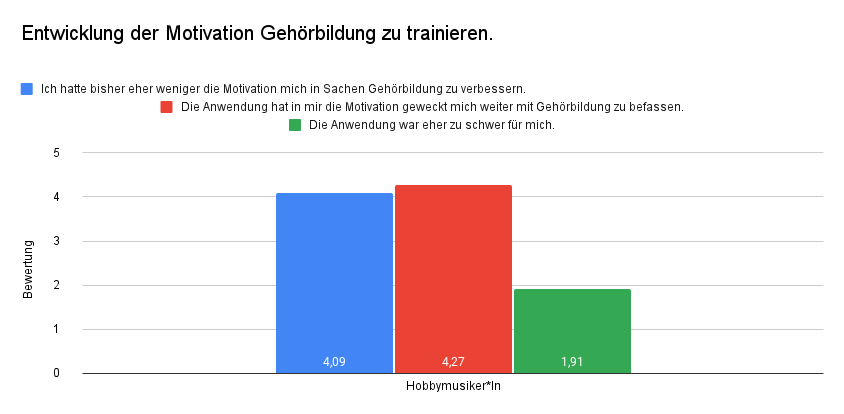
\includegraphics[width=1\textwidth]{Bilder/eval-entwicklungMotivationHobby-vergleich.png}
    \caption{Veränderung der Motivation der Hobbymusiker*Innen}
\end{figure}
Es lässt sich an der Abbildung gut erkennen, dass der Großteil der Hobbymusiker nie die Motivation hatten sich in Gehörbildung zu verbessern. Der Mittelwert der abgegebenen Bewertungen zu der Frage, ob man bisher eher weniger die Motivation hatte Gehörbildung zu trainieren, liegt bei 4.09. Dem entgegen liegt der Mittelwert der Bewertungen, ob man durch die Anwendung nun die Motivation erlangt hat sich weiter fortzubilden, bei 4.27. Man kann gut erkennen, dass die Motivation der Hobbymusiker gestiegen ist. Die erhöhte Motivation lässt sich dabei wahrscheinlich darauf zurückführen, dass der Großteil der Hobbymusiker die Schwierigkeit der Anwendung bei 1.91 bewertete. Die Schwierigkeit liegt dabei leicht unter einer mittleren Schwierigkeit, was wahrscheinlich dazu führte, dass sich die Musiker leicht gefordert fühlten, jedoch nicht überfordert. Weiterhin ergab sich, dass die meisten Hobbymusiker einen postiven Lerneffekt durch die Anwendung erfahren haben.  

\subsection*{Studierende}
\begin{figure}[H]
    \centering
    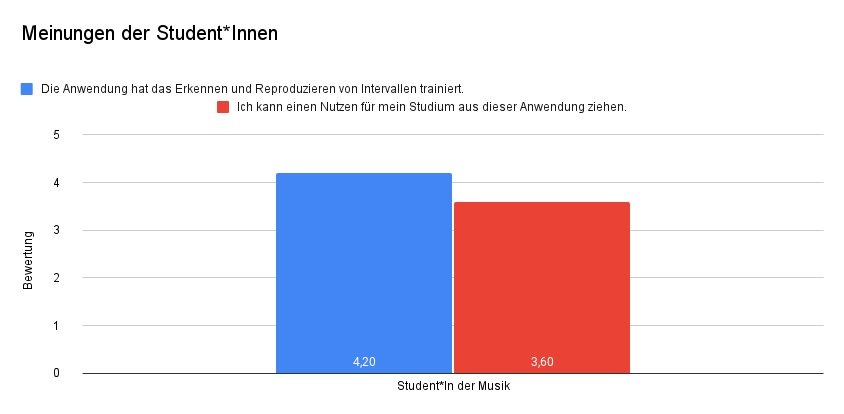
\includegraphics[width=1\textwidth]{Bilder/eval-meinungenStudis.png}
    \caption{Meinungen der Student*Innen}
\end{figure}
Die Meinungen der Studierenden zu der Anwendung sind vor allem Interessant im Hinblick auf das vermittelte Wissen. Der Unterschied zu Hobbymusikern liegt dabei ganz klar in der Erfahrung. Da Studierende bereits Gehörbildung im Studium üben müssen, haben diese einen ganz anderen Blickwinkel auf den gleichen Sachverhalt des vermittelten Wissens. Die Studierenden sagten so mit einer deutlichen Mehrheit aus, dass die Anwendung das Erkennen und Reproduzieren von Intervallen trainiert hat, mit einer Bewertung von 4.2. Weiterhin ergab die Befragung, dass die Studierenden mit einer Bewertung von 3.6 einen Nutzen aus der Anwendung für ihr Studium ziehen können. Es lässt sich also sagen, dass die Anwendung selbst Studierenden, welche eine akademische Ausbildung in der Gehörbildung erhalten, immer noch einen Vorteil und Nutzen in diesem Gebiet bietet. 

\subsection*{Professionelle Musiker}
\begin{figure}[H]
    \centering
    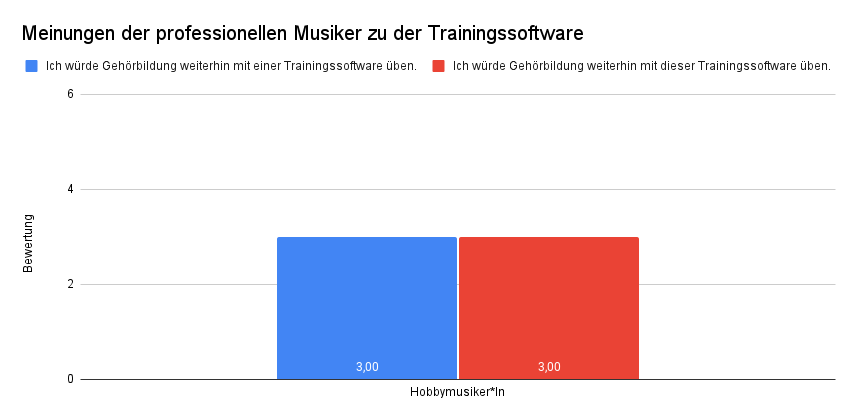
\includegraphics[width=1\textwidth]{Bilder/eval-profis.png}
    \caption{Meinung der professionellen Musiker zu Trainingssoftware}
\end{figure}
Die professionellen Musiker beantworteten die Frage, dass Gehörbildung wichtig in ihrem Alltag ist mit einer durchschnittlichen Bewertung von 4.67. Jedoch sagte nur eine Person, dass sie eine und noch eher die vorgestellte Trainingssoftware in der Zukunft verwenden würde. Die anderen beiden Personen erachten Trainingssoftware für Gehörbildung offenkundig als für nicht zielbringend. Im Durchschnitt geben die professionellen Musiker also ein neutrales Bild wieder.

\subsection*{Allgemeine Fragen}
Im folgenden Abschnitt soll es darum gehen, ob die gesetzten Ziele erreicht wurden. Dabei wird zwischen der Gesamtmeinung aller Tester und der Meinungen der Gruppen unterschieden. Es galt, eine Tonerkennung im Umfeld von Unity mit einer adäquaten Erkennungsrate zu entwickeln. Weiterhin sollte eine gute User Experience für den Nutzer designed und umgesetzt werden. 
\begin{figure}[H]
    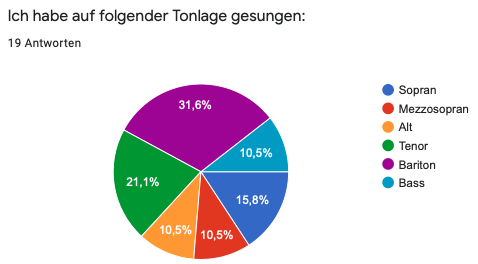
\includegraphics[width=0.45\textwidth]{Bilder/eval-tonart.png}
    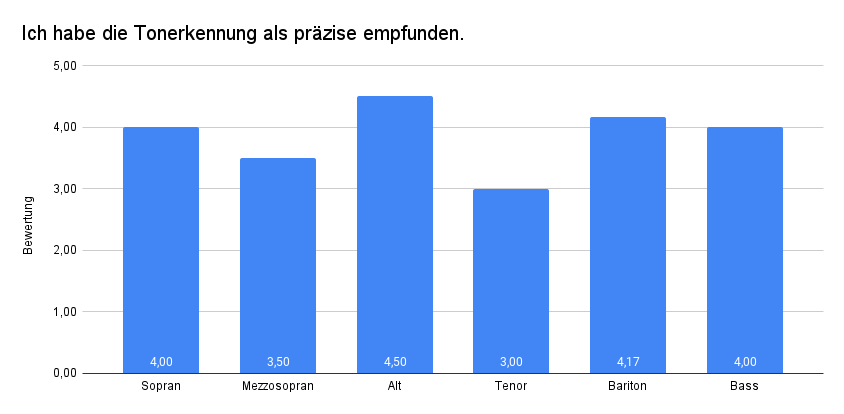
\includegraphics[width=0.55\textwidth]{Bilder/eval-tonerkennung-vergleichLagen.png}
    \caption{Abhängigkeit der Präzision der Tonerkennung von der Tonlage}
\end{figure}
Wie bereits angenommen in der Konzeption, zeigt sich in der Evaluation, dass die Tonerkennung schlechter performed, um so tiefer die Lage der Person ist. Die \glqq Damenstimmen'', hier die linken drei Balken, lassen sich im Durchschnitt besser erkennen, als die \glqq Herrenstimmen''. Dieser Zusammenhang lässt sich daher erklären, dass eine Herrenstimme oftmals eine Vielzahl an stark schwingenden Obertönen beinhält. Der vorgestellte Pitch Detection Algorithmus ist, wie in der Konzeption erwähnt, gegen zu starke Obertöne anfällig und ist zusätzlich schwer für eine solche obertonlastige Stimme einzustellen. Jedoch ist der Fehler des Pitch Detection Algorithmus nicht nur auf die Stimmlage begrenzt, wie man in der nächsten Grafik erkennen kann. 
\begin{figure}[H]
    \centering
    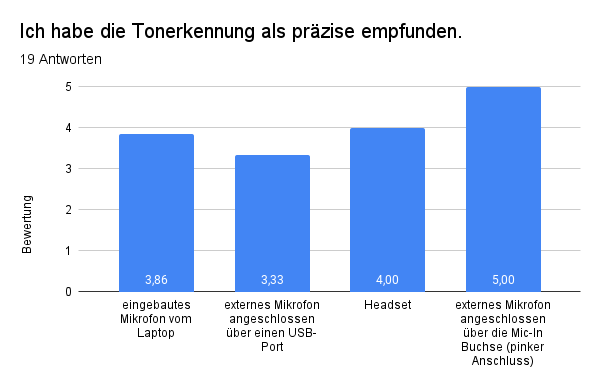
\includegraphics[width=1\textwidth]{Bilder/eval-tonerkennung-vergleichMikrofon.png}
    \caption{Abhängigkeit der Präzision der Tonerkennung von der Mikrofonart}
\end{figure}
Es lässt sich gut ablesen, dass die Tonerkennung bei einem Mikrofon, welche über den Mic-in Anschluss angeschlossen ist, besser abschneidet, als alle Anderen. Die Qualität eines über den Mic-in angeschlossenen Mikrofons ist oftmals besser, als eines, welches fest in einen Laptop verbaut ist. Hintergrundrauschen oder knacken, welches bei schlechteren Mikrofonen häufig ist, hat offensichtlich einen negativen Einfluss auf einen Pitch Detection Algorithmus. \\\\
Die Tonerkennung wurde nicht nur in Hinsicht auf die Erkennung allein konzipiert, sondern auch auf den echtzeit Aspekt. Die Erfahrungen zu der Performance sehen wie folgt aus.
\begin{figure}[H]
    \centering
    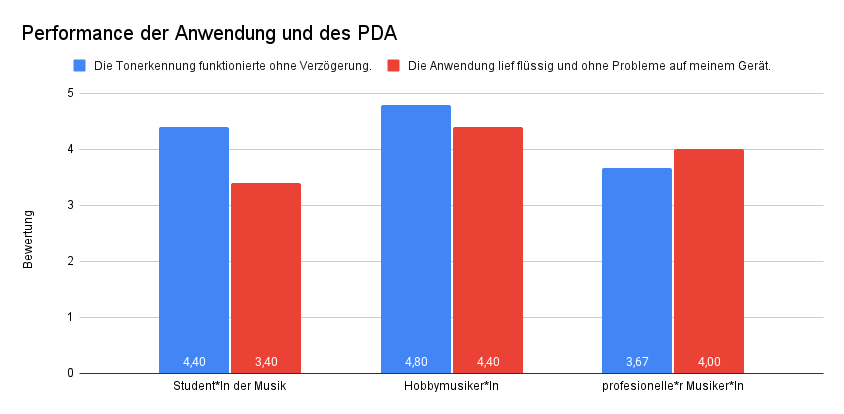
\includegraphics[width=1\textwidth]{Bilder/eval-verzoegerung-vergleich.png}
\end{figure} 
Alle Musikergruppen sagten in ähnlichem Maße aus, dass die Tonerkennung spezifisch ohne Verzögerung funktionierte. Weiterhin sagen ebenfalls alle Musikergruppen aus, dass die gesamte Anwendung flüssig läuft. Beide dieser Werte sind positive Aussagen über die echtzeit Erkennung des Tons und auch ein positiver Punkt für die User Experience. Weitere Ergebnisse zu der User Experience lassen sich aus dem Spaß der Nutzer, sowie der Bedienungsfreundlichkeit ableiten. 
\begin{figure}[H]
    \centering
    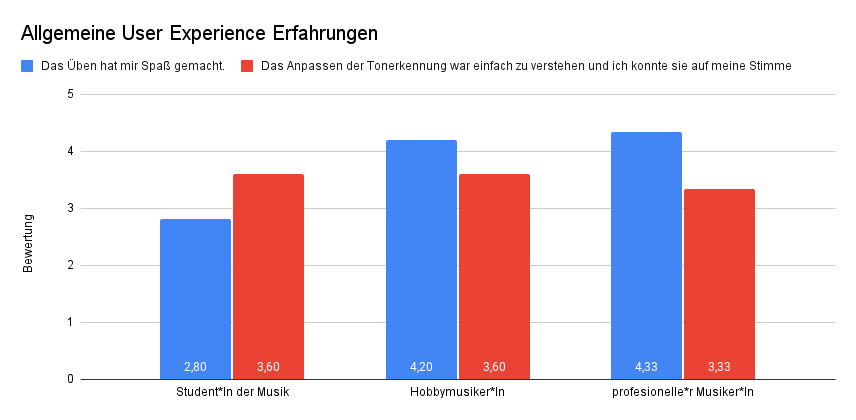
\includegraphics[width=1\textwidth]{Bilder/eval-zufriedenheitUX-vergleich.png}
\end{figure} 
So sagen zwei der drei Gruppen aus, dass ihnen das Üben mit der Anwendung Spaß gemacht hat. Weiterhin wird ausgesagt, dass das Anpassen der Tonerkennung auf die eigene Stimme in den meisten Fällen ebenfalls gut von statten ging. 

\chapter{Fazit und Ausblick}

Im Rahmen dieser Arbeit wurde ein Trainingsprogramm zur Schulung des Gehörs mit Unity implementiert. Der Fokus lag dabei vor allem auf der echtzeit Tonerkennung von gesungenen Tönen des Nutzers. Es wurde der aktuelle Stand der Trainingssoftware zur Schulung des Gehörs analysiert und auf dem Wissen der Analyse eine eigene Trainingssoftware konzipiert. Anschließend wurden Pitch Detection Algorithmen daraufhin analysiert, wie tauglich diese für eine Umsetzung in Unity sind. Wichtig war außerdem, dass die Tonerkennung in Echtzeit funktionieren würde. Es musste daher ebenfalls auf die Tonverarbeitung mit Unity Rücksicht genommen werden. \\
Die analysierten Trainingsprogramme sind zu einem Großteil veraltet und simpel gehaltene Lernprogramme zur Unterstützung des Lernenden. Kein untersuchtes Programm, mit der Ausnahme von einem, bietet dem Nutzer die Möglichkeit praktisch zu lernen. Die User Experience der State of the Art Anwendungen ist ebenfalls nicht ideal; die Anwendungen sind mehr als Lernhilfe konzipiert, statt als komplette Lernumgebung. Es fehlt ihnen häufig an einer anfängerfreundlichen Einführung, da sie vor allem für Studenten und fortgeschrittene Schüler konzipiert sind. Ein positives Beispiel der Analyse ist Earmaster, welches in fast allen Kritikpunkten die Ausnahme darstellt. \\
Die Audioverarbeitung mit Unity bietet nur eine Möglichkeit Daten aus dem Mikrofon einzulesen und weiterzuverarbeiten. Die untersuchten PDAs reichen von sehr naiven Ansätzen bis hin zu sehr mächtigen Laufzeitintensiven Algorithmen. Es wurde entschieden, einen eigenen Algorithmus auf dem erlangten Wissen zu konzipieren und zu implementieren. Das Trainingsprogramm wurde anschließend zunächst aus der Sicht der Nutzer konzipiert, wobei die User Experience und ein simples und übersichtliches Design im Vordergrund stand. Es wurde beschrieben, wie der Nutzer mit dem Interface agieren soll und was die generellen Kernaspekte des Spiels sein sollten. In der Konzipierung der Systemkomponenten wurde darauf eingegangen, wie die Anwendung implementiert werden sollte und wie die Komponenten untereinandern kommunizieren sollten. Die Konzipierung der Tonerkennung wurde in einem eigenen Unterkapitel behandelt, da diese einen Kernteil der Arbeit darstellt. \\
Die Implementierung von einer solchen Anwendung in Unity ist nicht ideal, da der Zugriff auf das Mikrofon und die weitere Verarbeitung der Daten nur in einer Art vonstattengehen kann. Dieser Umstand bietet starke Einschränkungen bei den möglichen Ansätzen, die verfolgt werden können. Der konzipierte Pitch Detection Algorithmus wurde dennoch mithilfe der einschränkenden Unity Funktionen implementiert. Wie sich in der Evaluation zeigt, funktioniert der PDA dennoch sehr gut. Die Tonerkennung funktioniert auf den tieferen Stimmlagen wie erwartet etwas schlechter, jedoch nie in einen negativ bewerteten Bereich. Allerdings zeigt dieser Verlauf, dass der PDA anfällig gegen Störgeräusche und Rauschen ist. Dieser Sachverhalt wird nochmal deutlicher in der Befragung zu dem verwendeten Mikrofon. Es muss angemerkt werden, dass sich gegen sehr robuste Ansätze entschieden wurde, da diese auch die rechenintensiven Ansätze sind. Wie sich ebenfalls in der Evaluation zeigte, lief die Anwendung und vor allem die Tonerkennung bei allen Testgruppen sehr performant und in Echtzeit. Der Lerneffekt der Anwendung wurde von den Studenten vor allem beurteilt; sie kommen zu der Aussage, dass das Trainingsprogramm das Erkennen von Intervallen trainiert hat. Die Anwendung hat jedoch nicht nur Wissen vermittelt, sondern nach der Aussage der Hobbymusiker und der professionellen Musiker, auch Spaß gemacht. Das Ziel, ein spielerisches Trainingsprogramm zur Gehörbildung zu entwickeln, wurde nach Aussage der Evaluation gut erreicht. Jedoch muss die vorliegende Arbeit unter dem Aspekt der limitierten Möglichkeiten von Unity betrachtet werden. Es ist wahrscheinlich, dass eine weitaus mächtigere Tonerkennung in einer anderen Gameengine umgesetzt werden könnte. 
Es gibt noch viele offene Fragen, welche sich mir stellen, da es trotz der erreichten Zielsetzung nicht zu einer idealen Umsetzung kam. \\\\
Wie sich bereits in der Evaluation zeigt, ist der PDA zwar gut, jedoch nicht perfekt. Es stellt sich mir die Frage, ob es nicht ähnlich oder besser performante Algorithmen gibt, welche trotzdem robuster sind und ähnlich eng in Unity verankert werden können. Es wäre weiterhin interessant, ein alleinstehendes Modul für Unity zu entwickeln, welches AudioClips auf ihre Töne hin untersucht und die jeweiligen Frequenzen zurückgibt. Ein solches Modul hätte nicht nur meine Arbeit erleichtert, ein Trainingsprogramm effizienter zu entwickeln, sondern würde es vielen anderen Entwicklern erleichtern ähnliche Programme zu schreiben. Wie in der Analyse deutlich wurde, fehlt es dem Gebiet der Trainingsanwendungen zur Schulung des Gehörs massiv an Innovation. Unity, als eine sehr flexible Umgebung zum Spiele entwickeln, würde mit einem solchen Tonerkennungsmodul die Möglichkeiten für Innovatoren eröffnen. Bleiben wir im Feld der möglichen Innovationen, so ist das Forschungsfeld der Tonerkennung mit Blick auf die Musik sehr breit. So könnten mögliche Ansätze zur Erweiterung einer Gehörbildungssoftware sein, dass durch verschiedene Machine Learning Ansätze eine Unterscheidung von einzelnen Stimmen oder Instrumenten vorgenommen wird, um so das Zusammenspiel mehrerer Musiker zu untersuchen. Weiterhin wäre es durchaus denkbar, eine Art KI Dirigenten zu entwickeln, welcher einem Ensemble dabei weiterhelfen könnte, ihr Zusammenspiel zu verbessern. Ebenso wäre es denkbar, dass dieses Programm einen Vergleich zu professionellen Orchestern herstellt, um so problematische Stellen des analysierten Vorspiels direkt in einer idealen Form vorzuspielen. \\
Abschließend lässt sich sagen, dass das Feld der Trainingsanwendungen zur Schulung des Gehörs noch großes Potential zeigt. Es gibt noch eine breites Anwendungsgebiet, welches von der Verbesserung der Lernerfahrung des Einzelnen bis hin zu komplett neuen Ideen, wie dem Untersuchen von ganzen Orchestern spannt. Große Vorreiter in diesem Gebiet sind nach wie vor das Team um \glqq Earmaster'' (\ref{sec:Earmaster}), welche diesen Bereich bereits seit 1994 voranbringen.



%- Zusammenfassung
%- Ausblick
%-- Offene Fragen? (Real time Erkennung, ...)
%--- Umsetzung für Chor? Machine Learning zur Unterscheidung? AI Dirigent?
%Literaturverzeichnis (APA)

	
	%======================================================
	% The back matter
	%======================================================
	%\cleardoublepage
	\refstepcounter{dummy}
	\addcontentsline{toc}{chapter}{\bibname}
	\bibliographystyle{alpha} % <--- layout of the bib
	\bibliography{bibliography.bib} % file name of your bib
	
	%======================================================
	% The optional appendix.
	%======================================================
	%\appendix
	%\addtocontents{toc}{\protect\setcounter{tocdepth}{0}}	
	%\input{appendix}
	
\end{document}
%======================================================
%======================================================
